\documentclass[healthcare,article,submit,pdftex,moreauthors]{Definitions/mdpi_es}

% Comandos internos de MDPI - no modificar
\firstpage{1}
\makeatletter
\setcounter{page}{\@firstpage}
\makeatother
\pubvolume{1}
\issuenum{1}
\articlenumber{0}
\pubyear{2026}
\copyrightyear{2026}
\datereceived{ }
\daterevised{ }
\dateaccepted{ }
\datepublished{ }

\graphicspath{{images/}}
\newcommand{\hoyes}{9 de octubre de 2026}

\AtBeginDocument{\renewcommand{\figurename}{Figura}\renewcommand{\tablename}{Tabla}\def\figureautorefname{Figura}\def\tableautorefname{Tabla}}
\usepackage{amsmath,amssymb,amsfonts}
\usepackage{graphicx}
\usepackage{float}
\usepackage{booktabs}
\usepackage{multirow}
\usepackage{tabularx}
\usepackage{array}
\usepackage{xcolor}
\usepackage{tikz}
\usetikzlibrary{shapes.geometric,arrows.meta,positioning,calc,backgrounds}
\AtBeginDocument{\doinum{}}
\makeatletter\@ifundefined{NC@find@L}{\newcolumntype{L}{>{\raggedright\arraybackslash}X}}{}\makeatother

% Marcadores rojos para elementos que los autores deben completar/confirmar antes del envío
\newcommand{\todo}[1]{\textcolor{red}{[\textbf{PENDIENTE:} #1]}}

\Title{Predicción de la mortalidad materna hospitalaria y de la morbilidad materna grave
       en MIMIC-IV mediante un ensamble apilado de aprendizaje automático
       bajo desbalance extremo de clases}

\newcommand{\orcidauthorA}{0009-0005-2358-4680}
\newcommand{\orcidauthorB}{0000-0003-0400-5020}

\Author{Emmanuel Gutiérrez Jiménez $^{1,}$*\orcidA{0009-0005-2358-4680}
        y José Duván Márquez Díaz $^{2}$\orcidB{0000-0003-0400-5020}}

\AuthorNames{Emmanuel Gutiérrez Jiménez y José Duván Márquez Díaz}

\address{%
$^{1}$ \quad Departamento de Ingeniería de Sistemas, Universidad del Norte,
              Barranquilla 081007, Colombia; emmanuelg@uninorte.edu.co\\
$^{2}$ \quad Departamento de Ingeniería de Sistemas, Universidad del Norte,
              Barranquilla 081007, Colombia; jmarquez@uninorte.edu.co}

\corres{Correspondencia: emmanuelg@uninorte.edu.co; Tel.: +57-310-432-6347}

\addhighlights{
\textbf{¿Cuáles son los principales hallazgos?}
\begin{itemize}
\item La muerte materna es demasiado infrecuente en MIMIC-IV para modelarla de forma
      confiable (41 de 25{,}736 ingresos obstétricos, 0.16\%): el AUC del ensamble
      apilado con validación cruzada de cinco particiones fue 0.857 $\pm$ 0.069, pero la precisión promedio fue de solo 0.156 $\pm$ 0.096.
\item Usar la morbilidad materna grave (MMG; 475 positivos, 1.85\%) como desenlace
      produjo una tarea notablemente más estable: en un conjunto de prueba independiente
      el ensamble apilado alcanzó un AUC de 0.913 y una precisión promedio de 0.384
      (unas 21 veces la prevalencia), con una sensibilidad de 0.79; la validación cruzada lo confirmó
      (AUC 0.904 $\pm$ 0.020, AP 0.419 $\pm$ 0.050). Marcar el 5\% superior de los ingresos
      capturó el 68\% de los casos de MMG.
\end{itemize}
\textbf{¿Cuáles son las implicaciones de los principales hallazgos?}
\begin{itemize}
\item En datos de un solo centro, la MMG es un objetivo de modelamiento más adecuado
      que la mortalidad para la predicción del riesgo materno; las estimaciones
      puntuales de mortalidad no deben sobreinterpretarse.
\item Retirar los indicadores de grupos diagnósticos del modelo de mortalidad redujo su AUC con
      validación cruzada de 0.857 a 0.725, y las probabilidades predichas no estuvieron calibradas
      (la recalibración de Platt posterior las corrigió): las puntuaciones brutas deben usarse para ordenar ingresos, y el riesgo absoluto solo tras recalibración y validación externa.
\item El sobremuestreo (SMOTE) no mejoró las métricas basadas en precisión, y la
      winsorización de valores atípicos evitó descartar el 19.5\% de las muertes y el
      38.7\% de los casos de MMG que la eliminación de filas habría removido.
\end{itemize}
}

\abstract{\textbf{Antecedentes}: La mortalidad materna sigue siendo una prioridad
mundial de salud, pero las muertes son tan infrecuentes en datos de un solo centro que
la evaluación estándar del aprendizaje automático (AA) resulta poco confiable. La
morbilidad materna grave (MMG; \emph{severe maternal morbidity}, SMM, en inglés),
definida mediante indicadores de diagnósticos y procedimientos de los CDC/HRSA, es
aproximadamente cien veces más frecuente y se emplea ampliamente como aproximación
al \emph{near miss}.
\textbf{Métodos}: Se construyeron dos modelos con la base de datos de historias
clínicas electrónicas MIMIC-IV a partir de 25{,}736 ingresos hospitalarios obstétricos
de mujeres de 12 a 55 años (rango observado: 18 a 55): el Modelo~A (muerte registrada durante el ingreso índice o
posteriormente; 41 eventos, 0.159\%) y el Modelo~B (al menos uno de los 20 indicadores
de MMG de la FAD-2023 de CDC/HRSA; 475 eventos, 1.846\%). El flujo de trabajo incluyó
limpieza de valores centinela y ceros implausibles, winsorización por rango
intercuartílico (RIC$\times$3) en lugar de eliminación de filas, imputación guiada por
la asimetría, escalado diferenciado e indicadores de diagnóstico agrupados por
expertos (usados únicamente en el Modelo~A para evitar fuga de información del
desenlace en el Modelo~B). Se ajustaron Random Forest, XGBoost, Extra Trees, regresión
logística y un ensamble apilado mediante búsqueda en malla con validación cruzada sobre
la precisión promedio. La validación cruzada estratificada de cinco particiones fue la
evidencia principal para el Modelo~A y complementó la evaluación en el conjunto de prueba del Modelo~B; se añadieron como análisis adicionales
SMOTE, un análisis del Modelo~A sin grupos diagnósticos, la calibración fuera de partición con bandas de riesgo, la recalibración de Platt e isotónica, los valores SHAP y una auditoría por subgrupos.
\textbf{Resultados}: Para el Modelo~A, el ensamble apilado alcanzó un AUC con validación
cruzada de 0.857 $\pm$ 0.069 y una precisión promedio (AP) de 0.156 $\pm$ 0.096
(prevalencia 0.0016); el conjunto de prueba contenía solo ocho muertes. Para el
Modelo~B, el ensamble apilado obtuvo el mejor AUC (0.913) y AP (0.384; prevalencia
0.018) en el conjunto de prueba, con sensibilidad de 0.79 y precisión de 0.14 con el
umbral predeterminado; restringido a hospitalizaciones por parto, la AP fue 0.646. La validación cruzada dio un AUC
de 0.904 $\pm$ 0.020 y una AP de 0.419 $\pm$ 0.050 para el Modelo~B, y marcar el 5\% superior de los
ingresos capturó el 68\% de los casos (valor predictivo positivo 0.25). Retirar los grupos diagnósticos redujo el
AUC con validación cruzada del Modelo~A de 0.857 a 0.725, las probabilidades predichas no estuvieron calibradas
(media 0.249 frente a una prevalencia de 0.018), pero la recalibración de Platt las corrigió (habilidad de Brier del Modelo~B de $-4.10$ a 0.26) y, en la auditoría por subgrupos, el AUC fue menor entre los
ingresos con estancia en UCI (0.655). SMOTE no mejoró la AP. \textbf{Conclusiones}: En esta cohorte de un solo centro, la MMG
permite una evaluación de AA considerablemente más estable que la mortalidad. Los
resultados siguen siendo exploratorios, porque la etiqueta de MMG se basa en códigos
CIE, los datos provienen de una sola institución y no se realizó validación externa.}

\keyword{mortalidad materna; morbilidad materna grave; \emph{near miss}; MIMIC-IV;
         ensamble apilado; desbalance de clases; precisión--sensibilidad;
         aprendizaje automático; historias clínicas electrónicas}

\begin{document}

%--------------------------------------------------------------------
\section{Introducción}
%--------------------------------------------------------------------
La mortalidad materna sigue siendo un problema importante de salud pública: la
Organización Mundial de la Salud y sus organismos aliados estimaron cerca de 287{,}000
muertes maternas en el mundo en 2020~\cite{WHO2023MMR}; los análisis de carga global siguen la mortalidad materna a lo largo del tiempo y entre regiones~\cite{Kassebaum2016GBD}, y un análisis sistemático de la OMS ha descrito sus principales causas~\cite{Say2014Causes}. Sin embargo, en hospitales de
altos recursos la muerte materna es un evento muy infrecuente. Esta rareza constituye un
obstáculo estadístico para el aprendizaje supervisado: con una prevalencia de unos pocos
casos por mil ingresos, cada partición de validación cruzada y cada conjunto de prueba
contienen apenas un puñado de positivos, de modo que un solo paciente mal clasificado
puede modificar la sensibilidad en varios puntos porcentuales, y la exactitud y el
AUC-ROC por sí solos dejan de ser informativos~\cite{Marshall2023Imbalance,Saito2015PR}.

Una forma ampliamente utilizada de mitigar este problema es modelar la
\emph{morbilidad materna grave} (MMG; SMM en inglés), o \emph{near miss}~\cite{Say2009NearMiss}, como
desenlace sustituto. Los Centros para el Control y la Prevención de Enfermedades de
Estados Unidos (CDC) definen la MMG mediante un conjunto de indicadores de
diagnósticos CIE-10-CM y de procedimientos CIE-10-PCS, que la Administración de
Recursos y Servicios de Salud (HRSA) distribuye en su documento de recursos de datos
federalmente disponibles (FAD)~\cite{CDC2023SMM,HRSA2023FAD}. Los eventos de MMG
ocurren aproximadamente cien veces más a menudo que las muertes maternas hospitalarias
entre las hospitalizaciones por parto y posparto~\cite{Callaghan2012SMM}, y se ha
mostrado que los códigos diagnósticos administrativos contienen información pronóstica
sobre la morbilidad materna~\cite{Clapp2021Prenatal}. La contrapartida es la calidad de
la etiqueta: una validación frente a la revisión de historias clínicas en un hospital
público reportó baja sensibilidad y bajo valor predictivo positivo para la
identificación de MMG basada en CIE-10~\cite{Boulet2024ICD10SMM}.

La base de datos MIMIC-IV, del Beth Israel Deaconess Medical Center y sucesora de MIMIC-III~\cite{Johnson2016MIMICIII}, ofrece registros
hospitalarios anonimizados con resultados de laboratorio, signos vitales registrados y
códigos diagnósticos~\cite{Johnson2023MIMICIV,Goldberger2000PhysioNet}. Aunque MIMIC-IV
no es una base de datos obstétrica, contiene miles de ingresos de mujeres con
diagnósticos relacionados con el embarazo, lo que permite una comparación reproducible
de las dos definiciones de desenlace sobre las mismas pacientes y los mismos
predictores.

El apilamiento de ensambles (\emph{stacking}) combina aprendices base heterogéneos
mediante un metaaprendiz y con frecuencia supera a sus componentes~\cite{Wolpert1992Stacking,Hastie2009ESL}.
Si esta ventaja persiste bajo un desbalance extremo, y si remedios habituales como el
sobremuestreo ayudan~\cite{vandenGoorbergh2022Harm}, es una cuestión empírica.
Este estudio hace, por tanto, las siguientes contribuciones:
\begin{itemize}[leftmargin=*,labelsep=5.8mm]
  \item Una comparación lado a lado de dos desenlaces en una misma cohorte obstétrica
        de 25{,}736 ingresos de MIMIC-IV: la muerte materna registrada en el ámbito
        hospitalario (Modelo~A) y la MMG definida por CDC/HRSA (Modelo~B).
  \item Un protocolo de evaluación consciente del desbalance: análisis ROC y de
        precisión--sensibilidad basado en probabilidades, precisión promedio como criterio
        de ajuste, validación cruzada estratificada como evidencia principal para el
        desenlace más infrecuente y un análisis de sensibilidad explícito con SMOTE.
  \item Control explícito de la fuga de información para la MMG: los indicadores de
        grupos diagnósticos derivados de los mismos códigos CIE que definen el desenlace
        se excluyen del Modelo~B, y un análisis de sensibilidad restringe la evaluación a
        las hospitalizaciones por parto (el denominador comparable con los CDC).
  \item Una política de valores atípicos basada en winsorización que conserva todos los
        casos positivos.
\end{itemize}
El resto del artículo se organiza como sigue. La Sección~\ref{sec:related}
revisa los trabajos relacionados, la Sección~\ref{sec:methods} describe los datos y los
métodos, la Sección~\ref{sec:results} presenta los resultados, la Sección~\ref{sec:discussion}
discute los hallazgos y las limitaciones, la Sección~\ref{sec:implications} considera las
implicaciones y el trabajo futuro, y la Sección~\ref{sec:conclusions} concluye.

%--------------------------------------------------------------------
\section{Trabajos relacionados}\label{sec:related}
\subsection{Aprendizaje automático para la morbilidad y mortalidad maternas}
Una revisión exploratoria de 39 estudios que aplicaron aprendizaje automático a datos de
historias clínicas electrónicas para predecir morbilidad y mortalidad maternas encontró
que los métodos de \emph{boosting} fueron el enfoque más utilizado (18 estudios), que los
desenlaces cardiovasculares e hipertensivos, la diabetes gestacional y la hemorragia
posparto fueron los objetivos más comunes, que muchos estudios carecían de validación
externa o de análisis de sensibilidad, que solo seis siguieron una guía de reporte y que
ninguno describió cómo se aplicaron los modelos en la práctica clínica~\cite{Vasudevan2025Scoping}.
La muerte materna rara vez es el desenlace modelado, y la predicción de desenlaces
perinatales ha sido revisada por separado por los autores~\cite{gutierrezjimenez2026artificial}. Los desenlaces perinatales, que comparten
fuentes de datos y algunos predictores con los maternos, se han modelado con más frecuencia: se han aplicado ensambles homogéneos a datos etíopes de salud materna y de
seguro de salud~\cite{Bogale2022Perinatal}, modelos de aprendizaje automático a un registro de nacimientos de Tanzania~\cite{Mboya2020Perinatal} y, en un registro de más de 500{,}000
embarazos de seis países de ingresos bajos y medios, modelos para mortinato y mortalidad neonatal alcanzaron un AUC de 0.71 o menos cuando solo se usó información
prenatal o previa al parto y superior a 0.80 en la mayoría de los modelos que incluyeron información del parto y del posparto~\cite{Shukla2020Perinatal}. Esta dependencia de la
discriminación respecto del momento en que se registran los predictores es relevante aquí, porque nuestros predictores también incluyen valores medidos durante el ingreso.

\subsection{Predicción de la morbilidad materna grave}
Los estudios sobre MMG son más numerosos porque el desenlace es más frecuente. Gao et al.\
desarrollaron un marco que identificó la MMG y sus factores de riesgo a partir de las
historias clínicas electrónicas de 45{,}858 partos en un centro médico académico; reportó un
AUC de 0.94 frente a 0.80 de un modelo basado en los CDC, y puso de manifiesto indicadores
como alteraciones electrolíticas, síndromes de respuesta inflamatoria y trastornos
ácido--base que no forman parte de la definición de los CDC~\cite{Gao2019SMM}. Li et al.\
predijeron la MMG definida por los CDC en 261{,}226 hospitalizaciones por parto en Maryland
(1{,}976 eventos; 76 por 10{,}000 partos) con regresión logística y LASSO, utilizando datos
vinculados de egresos hospitalarios y de encuestas hospitalarias; el mejor modelo, un LASSO
con 18 variables, alcanzó un AUC con validación cruzada de 0.796 con baja sensibilidad en
todos los modelos, y los autores reportaron un riesgo no ajustado aproximadamente el doble
para mujeres negras no hispanas en comparación con mujeres blancas no hispanas. Señalaron
el desbalance de clases y la falta de validación externa como limitaciones y propusieron
técnicas de sobremuestreo como SMOTE como trabajo futuro~\cite{Li2025Maryland}.
También se ha mostrado que los códigos diagnósticos registrados durante el control
prenatal contienen información pronóstica sobre la morbilidad materna~\cite{Clapp2021Prenatal}.

\subsection{Calidad de la etiqueta y metodología para eventos raros}
La confiabilidad de las etiquetas de MMG es una preocupación reconocida: la identificación
basada en CIE-10 se comparó con la revisión de historias clínicas en un hospital público y
mostró baja sensibilidad y bajo valor predictivo positivo~\cite{Boulet2024ICD10SMM}. Al mismo
tiempo, la MMG ocurre aproximadamente cien veces más a menudo que la muerte materna
hospitalaria~\cite{Callaghan2012SMM}, lo que la convierte en el sustituto habitual cuando
las muertes son demasiado pocas para modelarlas. El trabajo metodológico sobre eventos raros
advierte que la exactitud y el AUC-ROC pueden ser poco informativos y que son preferibles el
análisis de precisión--sensibilidad y el reporte explícito de la incertidumbre~\cite{Marshall2023Imbalance,Saito2015PR},
y que las correcciones del desbalance pueden perjudicar la calibración sin mejorar la
discriminación~\cite{vandenGoorbergh2022Harm}.

\subsection{Posicionamiento de este estudio}
Frente a los estudios anteriores, el presente trabajo se diferencia en cuatro aspectos.
Primero, utiliza como predictores signos vitales al ingreso y valores de laboratorio de todo el
hospital provenientes de MIMIC-IV, en lugar de datos de reclamaciones o de egresos. Segundo,
modela la mortalidad y la MMG sobre los \emph{mismos} 25{,}736 ingresos obstétricos con los mismos
predictores y el mismo flujo de trabajo, lo que permite una comparación directa de las dos
definiciones de desenlace. Tercero, controla explícitamente la fuga de información del
desenlace y reporta un análisis de sensibilidad solo de partos comparable con los CDC. Cuarto,
evalúa el remedio de sobremuestreo que Li et al.\ dejaron como trabajo futuro~\cite{Li2025Maryland},
utilizando SMOTE estrictamente dentro de las particiones de validación cruzada.

%--------------------------------------------------------------------
\section{Materiales y métodos}\label{sec:methods}
%--------------------------------------------------------------------
\subsection{Fuente de datos y cohorte de estudio}
Se utilizó MIMIC-IV alojada en PostgreSQL~\cite{Johnson2023MIMICIV}
(versión 3.1, publicada en PhysioNet en octubre de 2024; acceso credencializado, datos descargados el 18 de abril de 2025). La base de datos abarca pacientes admitidos al servicio de urgencias o a unidades de cuidados intensivos del Beth Israel Deaconess Medical Center entre 2008 y 2022, con todas las fechas desidentificadas mediante un desplazamiento específico por paciente.
La cohorte de estudio comprende ingresos hospitalarios de mujeres de 12 a 55 años (el rango observado fue de 18 a 55 años) con al
menos un diagnóstico CIE obstétrico o relacionado con el embarazo (posición del diagnóstico
$\leq 4$), identificados mediante un universo diagnóstico ampliado que combina la búsqueda de
texto en los títulos largos de CIE con rangos de códigos CIE. \emph{No} se exigió una estancia en
la unidad de cuidados intensivos (UCI): esto es importante porque 30 de las 41 muertes registradas
(73\%) ocurrieron en ingresos sin ninguna estancia en UCI. La cohorte final contiene
25{,}736 ingresos, de los cuales 8{,}857 se identificaron como hospitalizaciones por parto.
La Figura~\ref{fig:pipeline} resume el flujo de trabajo.

\begin{figure}[H]
\centering
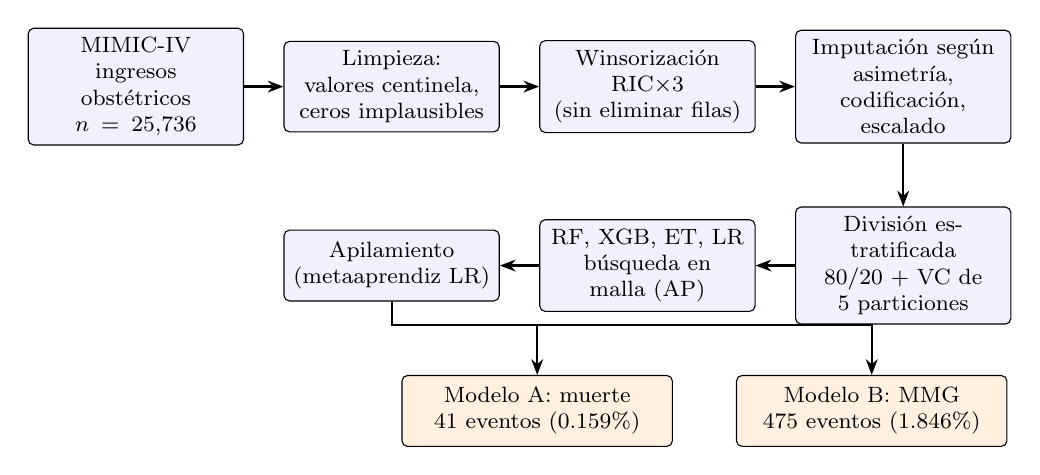
\begin{tikzpicture}[
  node distance=4mm and 5mm,
  box/.style={rectangle,draw,rounded corners=2pt,align=center,font=\footnotesize,
              minimum height=9mm,text width=2.5cm,fill=blue!6},
  outbox/.style={rectangle,draw,rounded corners=2pt,align=center,font=\footnotesize,
              minimum height=9mm,text width=3.2cm,fill=orange!12},
  arr/.style={-{Stealth[length=2mm]},thick}]
\node[box] (a) {MIMIC-IV\\ingresos obstétricos\\$n=25{,}736$};
\node[box,right=of a] (b) {Limpieza:\\valores centinela,\\ceros implausibles};
\node[box,right=of b] (c) {Winsorización\\RIC$\times$3\\(sin eliminar filas)};
\node[box,right=of c] (d) {Imputación según\\asimetría,\\codificación, escalado};
\node[box,below=8mm of d] (e) {División estratificada\\80/20 + VC de 5 particiones};
\node[box,left=of e] (f) {RF, XGB, ET, LR\\búsqueda en malla (AP)};
\node[box,left=of f] (g) {Apilamiento\\(metaaprendiz LR)};
\node[outbox,below=8mm of f,xshift=-14mm] (h) {Modelo A: muerte\\41 eventos (0.159\%)};
\node[outbox,right=8mm of h] (i) {Modelo B: MMG\\475 eventos (1.846\%)};
\draw[arr] (a)--(b); \draw[arr] (b)--(c); \draw[arr] (c)--(d);
\draw[arr] (d)--(e); \draw[arr] (e)--(f); \draw[arr] (f)--(g);
\draw[arr] (g.south)--++(0,-3mm)-|(h.north);
\draw[arr] (g.south)--++(0,-3mm)-|(i.north);
\end{tikzpicture}
\caption{Visión general del flujo de trabajo. Se aplican los mismos pasos de limpieza,
preprocesamiento y aprendizaje a ambos desenlaces. VC: validación cruzada.}\label{fig:pipeline}
\end{figure}

\subsection{Definiciones de los desenlaces}
\textbf{Modelo A (mortalidad).} El desenlace es 1 si se registró una hora de muerte
hospitalaria durante el ingreso índice o en cualquier ingreso posterior de la misma paciente,
y 0 en caso contrario. Esto produjo 41 eventos entre 25{,}736 ingresos (0.159\%).

\textbf{Modelo B (MMG).} Un ingreso es positivo para MMG si presenta al menos un código de
diagnóstico CIE-10-CM o de procedimiento CIE-10-PCS que coincida con alguno de los 20
indicadores vigentes de la FAD-2023 de CDC/HRSA~\cite{CDC2023SMM,HRSA2023FAD,Nebraska2024SMM}
(se excluye el antiguo indicador de transfusión de hemoderivados, retirado por la HRSA en 2023).
Los indicadores se agrupan en siete categorías clínicas (cardiaca, renal, respiratoria,
hemorragia, sepsis, otras obstétricas y otras médicas). Hubo 475 ingresos positivos para MMG
(1.846\%); entre las 8{,}857 hospitalizaciones por parto, 252 fueron positivas (2.845\%, es
decir, 284.5 por 10{,}000), por encima del rango de referencia publicado de 58--88 por 10{,}000
partos~\cite{Nebraska2024SMM}. La mayor tasa es esperable, pues MIMIC-IV es un centro de
referencia terciario y el denominador ampliado incluye también ingresos que no son partos.
Los indicadores más frecuentes fueron insuficiencia renal aguda (180 ingresos), choque (72),
SDRA (66), sepsis (62) y coagulación intravascular diseminada (61); el 23.4\% de los ingresos
positivos cumplió indicadores de más de una categoría clínica.

\subsection{Predictores y preprocesamiento}
Los predictores candidatos comprendieron variables administrativas (edad al ingreso, grupo
étnico, seguro de salud, grupo de idioma, tipo de ingreso, lugar de ingreso, estancia en UCI y
número de estancias en UCI) y el valor más temprano disponible de 27 variables de
registro/laboratorio (signos vitales, componentes de la escala de coma de Glasgow, hematología
y química). Para las 13 variables de laboratorio, los valores se tomaron también de los eventos
de laboratorio de todo el hospital (no solo de los eventos registrados en UCI), lo cual es
relevante aquí porque la mayoría de las muertes ocurrió fuera de la UCI. Los pasos de
preprocesamiento fueron:

\begin{enumerate}[leftmargin=*,labelsep=5.8mm]
\item \textbf{Valores centinela y ceros implausibles.} El marcador 999{,}999 y los ceros
      fisiológicamente imposibles se establecieron como faltantes.
\item \textbf{Manejo de valores atípicos mediante winsorización.} Para cada variable continua,
      los valores más allá de $Q_1 - 3\,\mathrm{RIC}$ o $Q_3 + 3\,\mathrm{RIC}$ se recortaron
      al límite más cercano (con cotas inferiores clínicas), de modo que ningún ingreso se
      elimina. Las escalas ordinales y las variables con $\mathrm{RIC}=0$ no se recortaron.
      Nuestra primera implementación eliminaba las filas con valores fuera de los límites,
      como en nuestro flujo de trabajo neonatal previo; una auditoría mostró que esto removía
      8 de 41 muertes (19.5\%) en el Modelo~A y 184 de 475 casos de MMG (38.7\%) en el Modelo~B,
      por lo que se reemplazó por la winsorización.
\item \textbf{Imputación.} Mediana para variables con $|\text{asimetría}|>1$, moda en caso
      contrario.
\item \textbf{Codificación y escalado.} Codificación \emph{one-hot} de los cinco grupos
      categóricos; \texttt{RobustScaler} para variables con $|\text{asimetría}|>1$ y
      \texttt{MinMaxScaler} en caso contrario. Las variables de monitoreo en UCI casi constantes
      (componente motor de la escala de Glasgow y Escala de Agitación--Sedación de Richmond; el
      valor más frecuente cubría más del 99\% de las filas) se descartaron del Modelo~A.
\end{enumerate}

\textbf{Indicadores de grupos diagnósticos y control de fuga de información.} Los códigos
diagnósticos CIE de la cohorte (4{,}116 códigos distintos para el Modelo~A) se agregaron en 26
indicadores binarios de grupos diagnósticos (\texttt{gdg\_m01}--\texttt{gdg\_m26}) según una
clasificación clínica realizada por un panel de cuatro expertos clínicos (un ginecólogo-obstetra con experiencia en medicina materno-fetal, un médico intensivista con experiencia en pacientes obstétricas, un especialista en medicina interna y un infectólogo) mediante un procedimiento estructurado de cuatro pasos.
Primero, se tabularon todos los códigos CIE de la cohorte por número y porcentaje de ingresos, y esta tabla de frecuencias fue el
documento de trabajo del panel. Segundo, los códigos suficientemente frecuentes como para identificar una entidad clínica bien definida
se conservaron como grupos individuales. Tercero, los códigos menos frecuentes fueron agrupados por los expertos según, en orden de
prioridad, un mecanismo fisiopatológico compartido, el sistema orgánico afectado y una relevancia pronóstica similar; ningún código se
asignó a más de un grupo y los desacuerdos se resolvieron mediante discusión hasta alcanzar consenso. Cuarto, el conjunto completo se revisó
en una sesión plenaria en cuanto a coherencia clínica, ausencia de superposición entre grupos y representación suficiente en la cohorte, y los
grupos que no cumplieron estos criterios se revisaron o fusionaron. Los códigos que no pudieron asignarse a un grupo clínicamente interpretable se
reservaron para un paso de agrupamiento residual.
Otros dos indicadores reservados para agrupamiento residual eran constantes y se eliminaron.
Dado que estos indicadores se derivan de los mismos diagnósticos codificados que definen la
MMG, se \emph{excluyeron} del Modelo~B; asimismo, los siete conteos de MMG por categoría, la
etiqueta multiclase y la bandera de hospitalización por parto no se usaron como predictores
(esta última se conserva únicamente para definir el subconjunto de evaluación).
El Modelo~A conservó los 26 indicadores, para un total de 89 predictores; el Modelo~B utilizó
65 predictores. Esta diferencia entre los conjuntos de predictores se considera en la
Sección~\ref{sec:discussion}.

La Tabla~\ref{tab:gdg} enumera los 26 grupos diagnósticos. De los 4{,}116 códigos CIE distintos
observados en la cohorte (2{,}192 CIE-10 y 1{,}924 CIE-9), 4{,}010 se asignaron a uno de los 26
grupos y 106 se excluyeron de la agrupación; doce grupos son obstétricos y catorce abarcan
afecciones no obstétricas. Un paso de k-medias destinado a agrupar los códigos residuales no
asignados no encontró códigos residuales, por lo que los dos indicadores de conglomerado
reservados eran constantes y se eliminaron.

\begin{table}[H]
\caption{Grupos diagnósticos utilizados como indicadores binarios en el Modelo~A: descripción,
si el grupo es obstétrico y número de códigos CIE distintos asignados.\label{tab:gdg}}
\small
\begin{tabularx}{\textwidth}{lLcc}
\toprule
\textbf{Indicador} & \textbf{Grupo} & \textbf{Obstétrico} & \textbf{Códigos CIE}\\
\midrule
gdg\_m01 & Complicaciones del trabajo de parto y del parto & Sí & 225 \\
gdg\_m02 & Afección preexistente que complica el embarazo & Sí & 167 \\
gdg\_m03 & Trastornos hipertensivos del embarazo & Sí & 95 \\
gdg\_m04 & Otros trastornos maternos relacionados con el embarazo & Sí & 83 \\
gdg\_m05 & Complicaciones fetales / gestación múltiple & Sí & 156 \\
gdg\_m06 & Otras complicaciones puerperales & Sí & 27 \\
gdg\_m07 & Trastornos de la placenta / del líquido amniótico & Sí & 43 \\
gdg\_m08 & Hemorragia (anteparto/posparto) & Sí & 57 \\
gdg\_m09 & Infección (obstétrica/puerperal) & Sí & 117 \\
gdg\_m10 & Trabajo de parto pretérmino / rotura prematura de membranas & Sí & 35 \\
gdg\_m11 & Aborto / embarazo ectópico o molar & Sí & 103 \\
gdg\_m12 & Trastornos venosos / tromboembólicos & Sí & 50 \\
gdg\_m13 & Neoplasias & No & 95 \\
gdg\_m14 & Enfermedades digestivas & No & 248 \\
gdg\_m15 & Trastornos endocrinos / metabólicos / nutricionales & No & 197 \\
gdg\_m16 & Enfermedades cardiovasculares & No & 231 \\
gdg\_m17 & Trastornos del sistema nervioso & No & 147 \\
gdg\_m18 & Enfermedades de la sangre / del sistema inmunitario & No & 107 \\
gdg\_m19 & Enfermedades genitourinarias (no obstétricas) & No & 175 \\
gdg\_m20 & Enfermedades respiratorias & No & 106 \\
gdg\_m21 & Factores administrativos / contacto con los servicios de salud & No & 306 \\
gdg\_m22 & Síntomas, signos y hallazgos mal definidos & No & 208 \\
gdg\_m23 & Enfermedades infecciosas y parasitarias & No & 147 \\
gdg\_m24 & Traumatismos, envenenamientos y causas externas & No & 355 \\
gdg\_m25 & Otras comorbilidades menores & No & 332 \\
gdg\_m26 & Trastornos mentales y del comportamiento & No & 198 \\
\bottomrule
\end{tabularx}
\end{table}

\subsection{Análisis de correlación}
La colinealidad se revisó en dos pasos: un mapa de calor de todas las variables clínicas
continuas y una revisión específica de los indicadores diagnósticos binarios, usando
$|r|\geq 0.70$ como umbral para un par fuertemente correlacionado. Dado que los aprendices
basados en árboles evalúan las variables de forma independiente en cada división y que la
regresión logística está regularizada con L2, se conservaron todas las variables
correlacionadas, ya que eliminar un miembro de una medición fisiológicamente pareada
descartaría señal monitorizada de forma independiente sin un beneficio de modelamiento.

\subsection{Algoritmos de aprendizaje y evaluación}
Se entrenaron Random Forest (RF), XGBoost (XGB), Extra Trees (ET) y regresión logística (LR)
con regularización L2 sobre una división estratificada 80/20 (semilla aleatoria 42):
20{,}588 ingresos de entrenamiento y 5{,}148 de prueba, con 33 y 8 muertes en el Modelo~A y
380 y 95 casos de MMG en el Modelo~B. El desbalance se manejó mediante ponderación de clases
(\texttt{balanced} o \texttt{balanced\_subsample}; \texttt{scale\_pos\_weight} de XGB de
622.9 en A y 53.2 en B). Los hiperparámetros se ajustaron con búsqueda en malla usando
validación cruzada estratificada de cinco particiones sobre el conjunto de entrenamiento, con
la \emph{precisión promedio} como criterio; las mallas fueron deliberadamente pequeñas para el
Modelo~A. Los aprendices ajustados se combinaron en un ensamble apilado~\cite{Wolpert1992Stacking}
con un metaaprendiz de regresión logística L2 ponderado por clases, cuyas entradas se generaron
con el mismo esquema estratificado de cinco particiones. La implementación utilizó scikit-learn,
XGBoost e imbalanced-learn~\cite{Pedregosa2011sklearn,Chen2016XGBoost,Chawla2002SMOTE}
con los modelos base RF~\cite{Breiman2001RF} y ET~\cite{Geurts2006ExtraTrees}. Los hiperparámetros seleccionados de cada aprendiz se presentan en la Tabla~\ref{tab:hyper}.

\begin{table}[H]
\caption{Hiperparámetros seleccionados (búsqueda en malla, validación cruzada estratificada de cinco particiones sobre la partición de entrenamiento, criterio: precisión promedio).
Ambos bosques usaron \texttt{max\_features} = sqrt; la ponderación de clases fue \texttt{balanced\_subsample} en RF y \texttt{balanced} en ET y LR.\label{tab:hyper}}
\small
\begin{tabularx}{\textwidth}{lXX}
\toprule
\textbf{Modelo} & \textbf{Modelo A (mortalidad)} & \textbf{Modelo B (MMG)}\\
\midrule
Random Forest & 400 árboles; profundidad máxima 20; división mínima 2; hoja mínima 2 & 300 árboles; profundidad máxima 20; división mínima 10; hoja mínima 4\\
XGBoost & 400 árboles; profundidad máxima 5; tasa de aprendizaje 0.1; submuestreo 0.8; muestreo de columnas 1.0; peso de la clase positiva 622.9 & 600 árboles; profundidad máxima 3; tasa de aprendizaje 0.01; submuestreo 0.8; muestreo de columnas 0.8; peso de la clase positiva 53.2\\
Extra Trees & 400 árboles; profundidad máxima sin límite; división mínima 2; hoja mínima 1 & 500 árboles; profundidad máxima 20; división mínima 10; hoja mínima 2\\
Regresión logística & L2; $C=0.01$; solver saga; 3{,}000 iteraciones & L2; $C=5$; solver lbfgs; 3{,}000 iteraciones\\
Apilamiento (metaaprendiz) & \multicolumn{2}{p{0.6\textwidth}}{Regresión logística L2; $C=0.1$; solver lbfgs; 5{,}000 iteraciones; ponderación de clases balanceada; entradas fuera de partición de cinco particiones}\\
\bottomrule
\end{tabularx}
\end{table}


Las curvas ROC y de precisión--sensibilidad (PR)~\cite{Fawcett2006ROC,Saito2015PR} y el AUC y la AP se calcularon a partir de las
probabilidades predichas de la clase positiva, mientras que el reporte de clasificación y la
matriz de confusión usaron el umbral de decisión predeterminado de 0.5. Dado que solo 8 muertes
caen en el conjunto de prueba del Modelo~A, la evidencia principal para este modelo es la
validación cruzada estratificada de cinco particiones sobre los 25{,}736 ingresos, reportada como
media $\pm$ desviación estándar para AUC, AP, sensibilidad, F1 y exactitud balanceada~\cite{Arlot2010CV}. Los criterios formales de tamaño de muestra para modelos de predicción dependen del número de predictores candidatos, de la prevalencia del desenlace y del desempeño esperado~\cite{Riley2020SampleSize}; con 41 eventos y 89 predictores candidatos (alrededor de 0.5 eventos por predictor), es poco probable que el Modelo~A los cumpla, lo que es una razón adicional para tratar sus resultados como exploratorios.
La validación cruzada reajusta las configuraciones ya ajustadas sobre el conjunto completo de datos;
por tanto, sus estimaciones son ligeramente optimistas, pues los hiperparámetros se seleccionaron
en la partición de entrenamiento. Como análisis de sensibilidad, SMOTE (estrategia de muestreo 0.2,
$k=5$) se ubicó dentro de cada partición de entrenamiento de un \emph{pipeline} para evitar fugas
hacia las particiones de validación. Para el Modelo~B, el ensamble apilado se evaluó además sobre el
subconjunto de hospitalizaciones por parto del conjunto de prueba, sin reentrenar.
El estudio sigue la guía de reporte TRIPOD+AI en lo aplicable~\cite{Collins2024TRIPODAI}
(la lista de verificación diligenciada se presenta como material suplementario).

\subsection{Análisis adicionales}\label{sec:additional}
Seis análisis adicionales complementan la evaluación principal.
(i)~\emph{Validación cruzada para el Modelo~B}: el mismo protocolo estratificado de cinco
particiones aplicado al Modelo~A se aplicó al Modelo~B, de modo que ambos desenlaces se evalúan con
la misma evidencia principal; una variante con SMOTE se ejecutó de la misma manera.
(ii)~\emph{Modelo~A sin grupos diagnósticos}: el Modelo~A se reevaluó mediante validación cruzada
tras retirar los 26 indicadores de grupos diagnósticos, conservando los hiperparámetros ajustados,
de modo que su conjunto de predictores coincida con el del Modelo~B.
(iii)~\emph{Calibración y estratificación del riesgo}: se utilizaron las probabilidades fuera de
partición (\emph{out-of-fold}) del ensamble apilado sobre toda la cohorte para calcular el puntaje de Brier~\cite{Brier1950} y su habilidad relativa a un modelo que predice la prevalencia, la razón entre la probabilidad
media predicha y la prevalencia observada, una curva de confiabilidad con intervalos por cuantiles~\cite{VanCalster2019Calibration,Guo2017Calibration} y
tablas de ``marcar el $x$\% superior'' con sensibilidad, valor predictivo positivo y \emph{lift}. Las
bandas de riesgo se definieron a partir de los percentiles de probabilidad del propio modelo (bajo:
por debajo del percentil 80; moderado: del 80 al 95; alto: 5\% superior), porque los puntos de corte
fijos carecen de sentido con estas prevalencias, y se calcularon intervalos de confianza del 95\%
mediante \emph{bootstrap} (500 remuestreos).
(iv)~\emph{Explicabilidad}: se calcularon valores TreeSHAP~\cite{Lundberg2017SHAP,Lundberg2020TreeSHAP} del aprendiz base XGBoost ajustado sobre
el conjunto de prueba del Modelo~B.
(v)~\emph{Auditoría por subgrupos}: el desempeño en el conjunto de prueba del ensamble apilado del
Modelo~B se describió por grupo étnico, seguro de salud, cuartil de edad, estancia en UCI e ingreso por
parto frente a no parto, reportando el AUC con intervalos de confianza \emph{bootstrap} solo para los
subgrupos con al menos 10 ingresos positivos y 10 negativos. Auditar el desempeño por subgrupos responde a preocupaciones documentadas de que los algoritmos pueden reproducir o amplificar inequidades en la atención en salud~\cite{Obermeyer2019Bias,Rajkomar2018Fairness}.
(vi)~\emph{Recalibración}: dado que la ponderación de clases infla las probabilidades predichas, se ajustaron el escalamiento de Platt (una regresión logística sobre el logit de la probabilidad del ensamble apilado) y la regresión isotónica sobre las probabilidades fuera de partición, dentro de una validación cruzada de cinco particiones repetida 20 veces y sin reentrenar los modelos, y se evaluaron con el puntaje de Brier y su habilidad, la razón entre la probabilidad media predicha y la prevalencia, el error de calibración esperado (ECE, diez intervalos por cuantiles), la pendiente y el intercepto de calibración, el AUC y la AP.

%--------------------------------------------------------------------
\section{Resultados}\label{sec:results}
%--------------------------------------------------------------------
\subsection{Cohortes y desenlaces}
La Tabla~\ref{tab:cohort} compara las dos tareas de predicción. El Modelo~B tiene 11.6 veces
más eventos que el Modelo~A y 95 positivos, en lugar de 8, en el conjunto de prueba.

\begin{table}[H]
\caption{Comparación de las dos tareas de predicción (los mismos 25{,}736 ingresos).\label{tab:cohort}}
\newcolumntype{C}{>{\centering\arraybackslash}X}
\begin{tabularx}{\textwidth}{lCC}
\toprule
 & \textbf{Modelo A (mortalidad)} & \textbf{Modelo B (MMG)}\\
\midrule
Ingresos positivos & 41 (0.159\%) & 475 (1.846\%)\\
Positivos en la división de entrenamiento / prueba & 33 / 8 & 380 / 95\\
Predictores & 89 (incl.\ 26 grupos diagnósticos) & 65 (sin grupos diagnósticos)\\
Peso de la clase positiva (XGBoost) & 622.9 & 53.2\\
Positivos retenidos tras el manejo de valores atípicos & 41 de 41 & 475 de 475\\
\bottomrule
\end{tabularx}
\end{table}

\subsection{Análisis descriptivo de la morbilidad materna grave}
Los 20 indicadores de CDC/HRSA se observaron al menos una vez. La Tabla~\ref{tab:smm} enumera el
número de ingresos por indicador. Los indicadores renales fueron la categoría más frecuente
(180 ingresos con al menos un indicador renal), seguidos de hemorragia (131),
respiratorios (89), otros médicos (77), sepsis (62), cardiacos (61) y otros obstétricos
(56). Cuando cada ingreso con MMG se asignó a la categoría con más
indicadores, las categorías primarias fueron renal (132), hemorragia (115), otros médicos
(71), cardiaca (52), otros obstétricos (38), respiratoria (36) y sepsis (31).
La mayoría de los ingresos con MMG involucró una sola categoría clínica (364 de 475, 76.6\%), mientras que 64
involucraron dos, 27 tres, 17 cuatro y 3 cinco categorías (111 ingresos, 23.4\%, con más de
una categoría). Los pares más frecuentes fueron respiratoria con hemorragia (42 ingresos), renal con
hemorragia (37), renal con respiratoria (28), cardiaca con respiratoria (26) y
hemorragia con sepsis (20) (Figura~\ref{fig:smmdesc}). La tasa de MMG fue de 184.6 por 10{,}000
ingresos en la cohorte ampliada y de 284.5 por 10{,}000 en las hospitalizaciones por parto, frente a
un rango publicado de 58--88 por 10{,}000 partos.

\begin{table}[H]
\caption{Ingresos por indicador de MMG de CDC/HRSA, agrupados por categoría clínica
(un ingreso puede contener varios indicadores).\label{tab:smm}}
\small
\begin{tabularx}{\textwidth}{lLc}
\toprule
\textbf{Categoría} & \textbf{Indicador} & \textbf{Ingresos}\\
\midrule
\multirow{6}{*}{Cardiaca} & Edema pulmonar / insuficiencia cardiaca aguda & 45\\
 & Conversión del ritmo cardiaco & 8\\
 & Infarto agudo de miocardio & 7\\
 & Paro cardiaco / fibrilación ventricular & 7\\
 & Aneurisma & 5\\
 & Insuficiencia / paro cardiaco durante cirugía o procedimiento & 1\\
\midrule
\multirow{3}{*}{Hemorragia} & Choque & 72\\
 & Coagulación intravascular diseminada & 61\\
 & Histerectomía & 41\\
\midrule
\multirow{2}{*}{Otras médicas} & Trastornos cerebrovasculares puerperales & 55\\
 & Anemia falciforme con crisis & 23\\
\midrule
\multirow{4}{*}{Otras obstétricas} & Embolia gaseosa y trombótica & 33\\
 & Eclampsia & 16\\
 & Embolia de líquido amniótico & 4\\
 & Complicaciones graves de la anestesia & 4\\
\midrule
Renal & Insuficiencia renal aguda & 180\\
\midrule
\multirow{3}{*}{Respiratoria} & Síndrome de dificultad respiratoria aguda & 66\\
 & Ventilación & 51\\
 & Traqueostomía temporal & 1\\
\midrule
Sepsis & Sepsis & 62\\
\bottomrule
\end{tabularx}
\end{table}
\unskip
\begin{figure}[H]
\centering
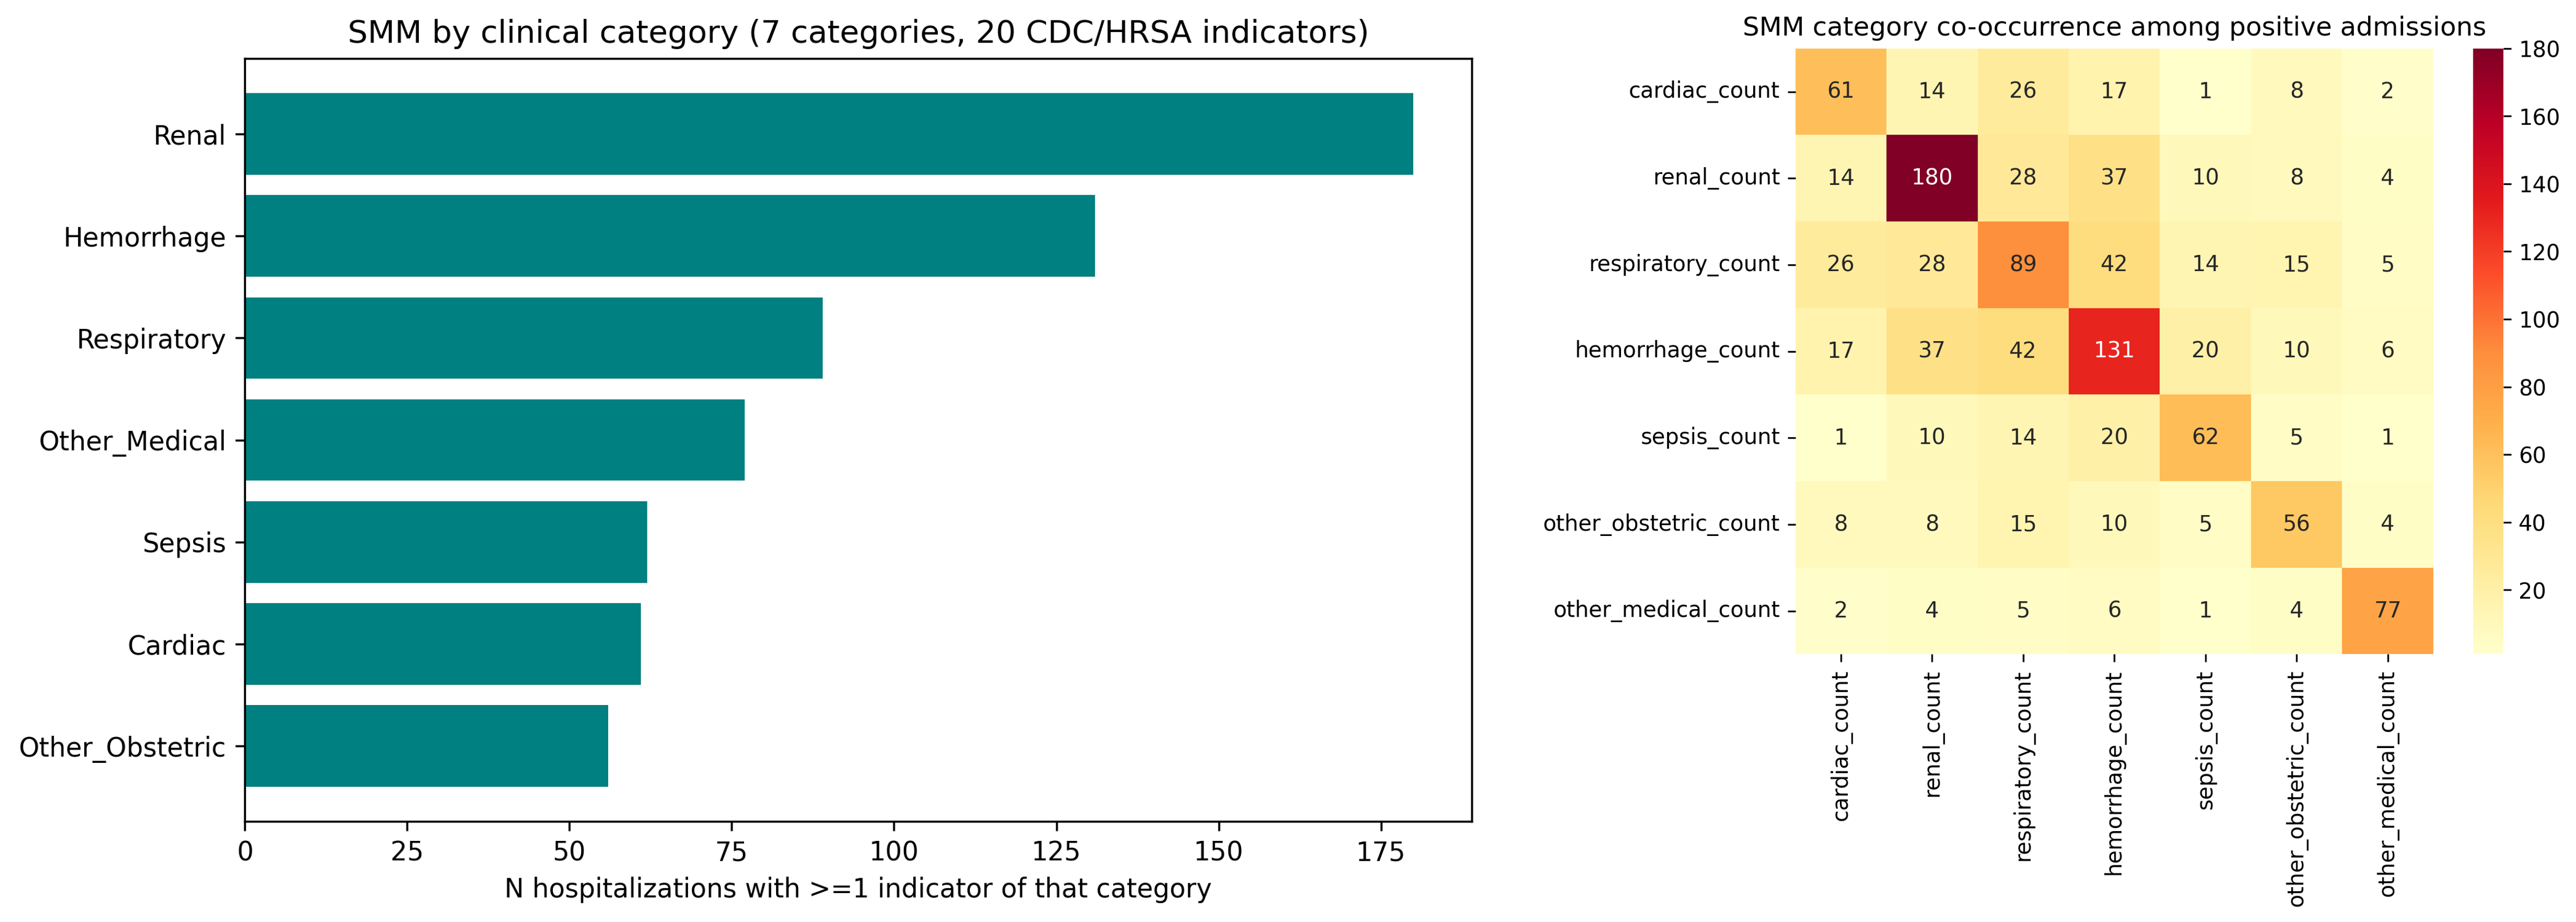
\includegraphics[width=\textwidth]{fig_smm_descriptive.png}
\caption{Ingresos con MMG por categoría clínica (izquierda) y coocurrencia de categorías entre los
ingresos con MMG (derecha; la diagonal indica el número de ingresos por categoría). Las
etiquetas de la figura están en inglés.}\label{fig:smmdesc}
\end{figure}

\subsection{Estructura de correlación de los predictores}
Diez pares de variables clínicas tuvieron $|r|\geq 0.70$ (Tabla~\ref{tab:corr}), todos
fisiológicamente esperables: estancia en UCI y número de estancias en UCI, las tres medidas de presión
arterial, los componentes de la escala de coma de Glasgow con la Escala de Agitación--Sedación de
Richmond, y hemoglobina con hematocrito. Siguiendo la política de la Sección~\ref{sec:methods}, no se
eliminó ninguna variable por colinealidad. El componente motor de Glasgow y la escala de Richmond se
descartaron del Modelo~A por varianza casi nula (valor más frecuente en más del 99\% de las filas) y se
conservaron en el Modelo~B.

\begin{table}[H]
\caption{Pares de variables clínicas con $|r|\geq 0.70$ (idénticos en ambos modelos).\label{tab:corr}}
\begin{tabularx}{\textwidth}{llc}
\toprule
\textbf{Variable 1} & \textbf{Variable 2} & \textbf{$r$}\\
\midrule
Estancia en UCI & Número de estancias en UCI & 0.958\\
Presión arterial media & Presión arterial diastólica & 0.907\\
Apertura ocular (Glasgow) & Respuesta verbal (Glasgow) & 0.891\\
Apertura ocular (Glasgow) & Respuesta motora (Glasgow) & 0.882\\
Hemoglobina & Hematocrito & 0.839\\
Presión arterial media & Presión arterial sistólica & 0.833\\
Apertura ocular (Glasgow) & Escala de Agitación--Sedación de Richmond & 0.783\\
Respuesta verbal (Glasgow) & Respuesta motora (Glasgow) & 0.773\\
Respuesta verbal (Glasgow) & Escala de Agitación--Sedación de Richmond & 0.754\\
Respuesta motora (Glasgow) & Escala de Agitación--Sedación de Richmond & 0.747\\
\bottomrule
\end{tabularx}
\end{table}

\subsection{Modelo A: mortalidad}
La Tabla~\ref{tab:cvA} y la Figura~\ref{fig:cvA} muestran los resultados con validación cruzada.
El ensamble apilado tuvo el AUC más alto (0.857 $\pm$ 0.069) y la mayor exactitud balanceada y
sensibilidad (0.780 y 0.731), pero su F1 fue de solo
0.014, y su AP (0.156 $\pm$ 0.096) fue menor que la de XGB y ET
(0.165 y 0.190), aunque dentro de una desviación estándar de ambas, y muy inferior a cualquier nivel clínicamente útil en términos absolutos, aunque
equivale aproximadamente a cien veces la prevalencia de 0.0016. La variabilidad entre particiones
fue grande (la desviación estándar de la AP llegó a 0.119 en XGB y a 0.096 en el ensamble apilado) y
RF no produjo predicciones positivas con el umbral predeterminado (sensibilidad 0). LR tuvo el menor
AUC y AP (0.758 y 0.049). En el conjunto de prueba (8
muertes), los valores de AUC variaron de 0.786 (RF) a 0.858 (XGB y ET), con el ensamble apilado
en 0.844 y una AP de 0.148, mientras que XGB tuvo la AP más alta (0.278) (Tabla~\ref{tab:holdout}). La matriz de confusión del ensamble apilado
contenía 7 verdaderos positivos, 1 falso negativo, 799 falsos positivos y 4{,}341 verdaderos
negativos (sensibilidad 0.88, precisión 0.009); estas estimaciones puntuales se basan en ocho
pacientes y deben leerse solo como ilustrativas.

\begin{table}[H]
\caption{Modelo~A: validación cruzada estratificada de cinco particiones (media $\pm$ DE) sobre los
25{,}736 ingresos (41 muertes).\label{tab:cvA}}
\scriptsize
\setlength{\tabcolsep}{3pt}
\begin{tabularx}{\textwidth}{lCCCCC}
\toprule
\textbf{Modelo} & \textbf{AUC} & \textbf{AP} & \textbf{Sensibilidad} & \textbf{F1} & \textbf{Exact.\ bal.}\\
\midrule
Random Forest & 0.809 $\pm$ 0.042 & 0.115 $\pm$ 0.091 & 0.000 $\pm$ 0.000 & 0.000 $\pm$ 0.000 & 0.500 $\pm$ 0.000\\
XGBoost & 0.817 $\pm$ 0.045 & 0.165 $\pm$ 0.119 & 0.117 $\pm$ 0.145 & \textbf{0.137 $\pm$ 0.172} & 0.558 $\pm$ 0.073\\
Extra Trees & 0.831 $\pm$ 0.051 & 0.190 $\pm$ 0.086 & 0.050 $\pm$ 0.061 & 0.089 $\pm$ 0.109 & 0.525 $\pm$ 0.031\\
Regresión logística & 0.758 $\pm$ 0.065 & 0.049 $\pm$ 0.058 & 0.631 $\pm$ 0.213 & 0.012 $\pm$ 0.004 & 0.735 $\pm$ 0.101\\
Apilamiento & 0.857 $\pm$ 0.069 & 0.156 $\pm$ 0.096 & \textbf{0.731 $\pm$ 0.124} & 0.014 $\pm$ 0.002 & \textbf{0.780 $\pm$ 0.058}\\
\bottomrule
\end{tabularx}
\end{table}
\unskip
\begin{figure}[H]
\centering
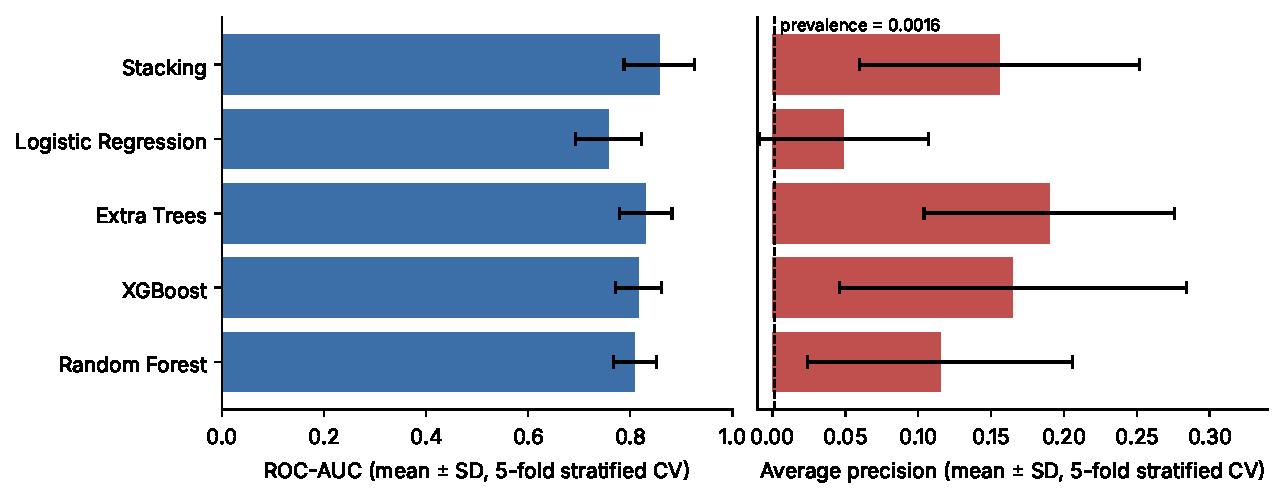
\includegraphics[width=0.85\textwidth]{fig_cv_modelA.pdf}
\caption{Modelo~A: AUC y precisión promedio con validación cruzada, con desviaciones estándar.
La línea discontinua marca la prevalencia del desenlace (41/25{,}736). Las etiquetas de la figura
están en inglés.}\label{fig:cvA}
\end{figure}

\subsection{Análisis de sensibilidad con sobremuestreo (Modelo A)}
Añadir SMOTE dentro de cada partición de entrenamiento aumentó el AUC de los cinco modelos
(p. ej., apilamiento de 0.857 a 0.870, XGB de 0.817 a 0.854, ET de 0.831 a 0.848) y la sensibilidad de RF, XGB
y ET, pero no la del ensamble apilado (de 0.731 a 0.142) ni la de LR (de 0.631 a 0.267).
La AP cambió poco: aumentó en apilamiento (de 0.156 a 0.168), XGB (de 0.165 a 0.173), RF (de 0.115 a 0.128)
y LR (de 0.049 a 0.052) y disminuyó en ET (de 0.190 a 0.173)
(Tabla~\ref{tab:smote}, Figura~\ref{fig:smote}). Los cambios en AUC y AP son todos menores que una
desviación estándar, mientras que la sensibilidad del ensamble apilado cayó de forma marcada. Dado que
el sobremuestreo principalmente desplaza el punto de operación en lugar de aportar información, y que
la AP no mejoró más allá del ruido entre particiones, se mantuvo la ponderación de clases como opción
predeterminada.

\begin{table}[H]
\caption{Modelo~A: efecto de SMOTE (estrategia de muestreo 0.2) sobre el AUC, la AP y la sensibilidad
con validación cruzada de cinco particiones (valores medios).\label{tab:smote}}
\small
\begin{tabularx}{\textwidth}{lCCCCCC}
\toprule
 & \multicolumn{2}{c}{\textbf{AUC}} & \multicolumn{2}{c}{\textbf{AP}} & \multicolumn{2}{c}{\textbf{Sensibilidad}}\\
\cmidrule(lr){2-3}\cmidrule(lr){4-5}\cmidrule(lr){6-7}
\textbf{Modelo} & Pesos & SMOTE & Pesos & SMOTE & Pesos & SMOTE\\
\midrule
Random Forest & 0.809 & 0.842 & 0.115 & 0.128 & 0.000 & 0.097\\
XGBoost & 0.817 & 0.854 & 0.165 & 0.173 & 0.117 & 0.142\\
Extra Trees & 0.831 & 0.848 & 0.190 & 0.173 & 0.050 & 0.097\\
Regresión logística & 0.758 & 0.809 & 0.049 & 0.052 & 0.631 & 0.267\\
Apilamiento & 0.857 & 0.870 & 0.156 & 0.168 & 0.731 & 0.142\\
\bottomrule
\end{tabularx}
\end{table}
\unskip
\begin{figure}[H]
\centering
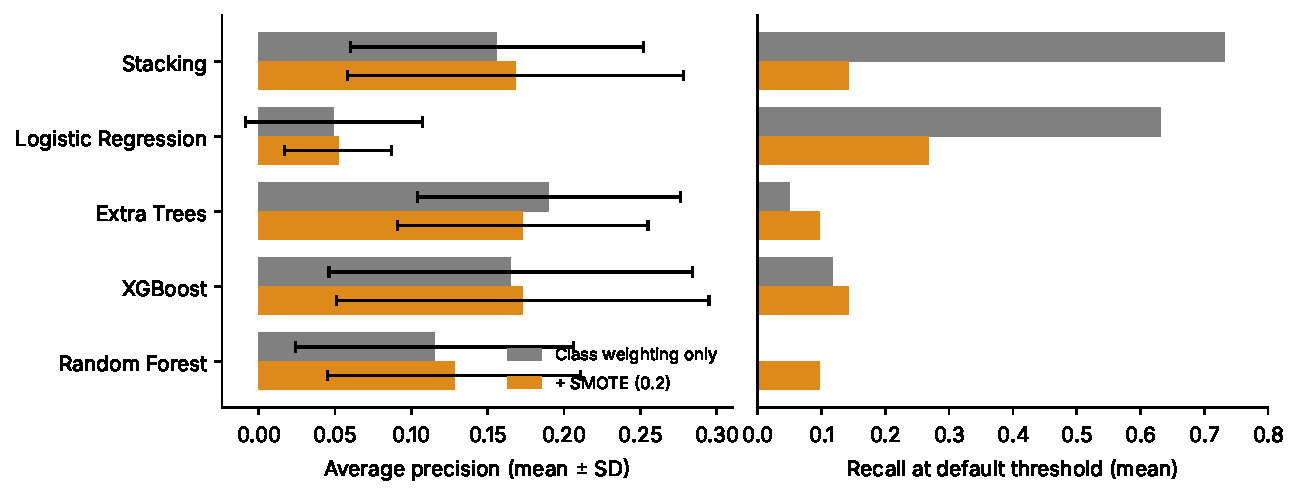
\includegraphics[width=0.95\textwidth]{fig_smote_modelA.pdf}
\caption{Modelo~A: ponderación de clases frente a SMOTE en validación cruzada de cinco particiones.
Las etiquetas de la figura están en inglés.}\label{fig:smote}
\end{figure}

\subsection{Modelo B: morbilidad materna grave}
El Modelo~B mostró un comportamiento mejor y mucho más estable. En el conjunto de prueba
(95 casos de MMG), el ensamble apilado fue el mejor modelo tanto en AUC (0.913) como en
AP (0.384), seguido de XGB (AUC 0.909, AP 0.358) y RF (AUC 0.900, AP 0.360)
(Tabla~\ref{tab:holdout}). La AP del ensamble apilado es unas 21 veces la
prevalencia en el conjunto de prueba (0.018). Con el umbral predeterminado, su matriz de confusión mostró 75
verdaderos positivos, 20 falsos negativos, 473 falsos positivos y 4{,}580 verdaderos negativos
(sensibilidad 0.79, precisión 0.14). Restringido a los 1{,}802 ingresos de prueba que fueron
hospitalizaciones por parto (58 casos de MMG, 3.219\%), el mismo modelo alcanzó una sensibilidad
de 0.78, precisión de 0.27, F1 de 0.40 para la clase positiva y una AP de 0.646
(frente a 0.384 en todo el conjunto de prueba), con una exactitud global de 0.93. La Figura~\ref{fig:rocpr}
muestra las curvas ROC y PR del ensamble apilado para ambos modelos.

\begin{table}[H]
\caption{Desempeño en el conjunto de prueba (probabilidades de la clase positiva): AUC y
precisión promedio. Conjunto de prueba del Modelo~A: 5{,}148 ingresos, 8 muertes; conjunto de prueba
del Modelo~B: 5{,}148 ingresos, 95 casos de MMG.\label{tab:holdout}}
\begin{tabularx}{\textwidth}{lCCCC}
\toprule
 & \multicolumn{2}{c}{\textbf{Modelo A (mortalidad)}} & \multicolumn{2}{c}{\textbf{Modelo B (MMG)}}\\
\cmidrule(lr){2-3}\cmidrule(lr){4-5}
\textbf{Modelo} & AUC & AP & AUC & AP\\
\midrule
Random Forest & 0.786 & 0.065 & 0.900 & 0.360\\
XGBoost & \textbf{0.858} & \textbf{0.278} & 0.909 & 0.358\\
Extra Trees & \textbf{0.858} & 0.161 & 0.900 & 0.315\\
Regresión logística & 0.854 & 0.031 & 0.889 & 0.339\\
Apilamiento & 0.844 & 0.148 & \textbf{0.913} & \textbf{0.384}\\
\bottomrule
\end{tabularx}
\end{table}
\unskip
\begin{figure}[H]
\centering
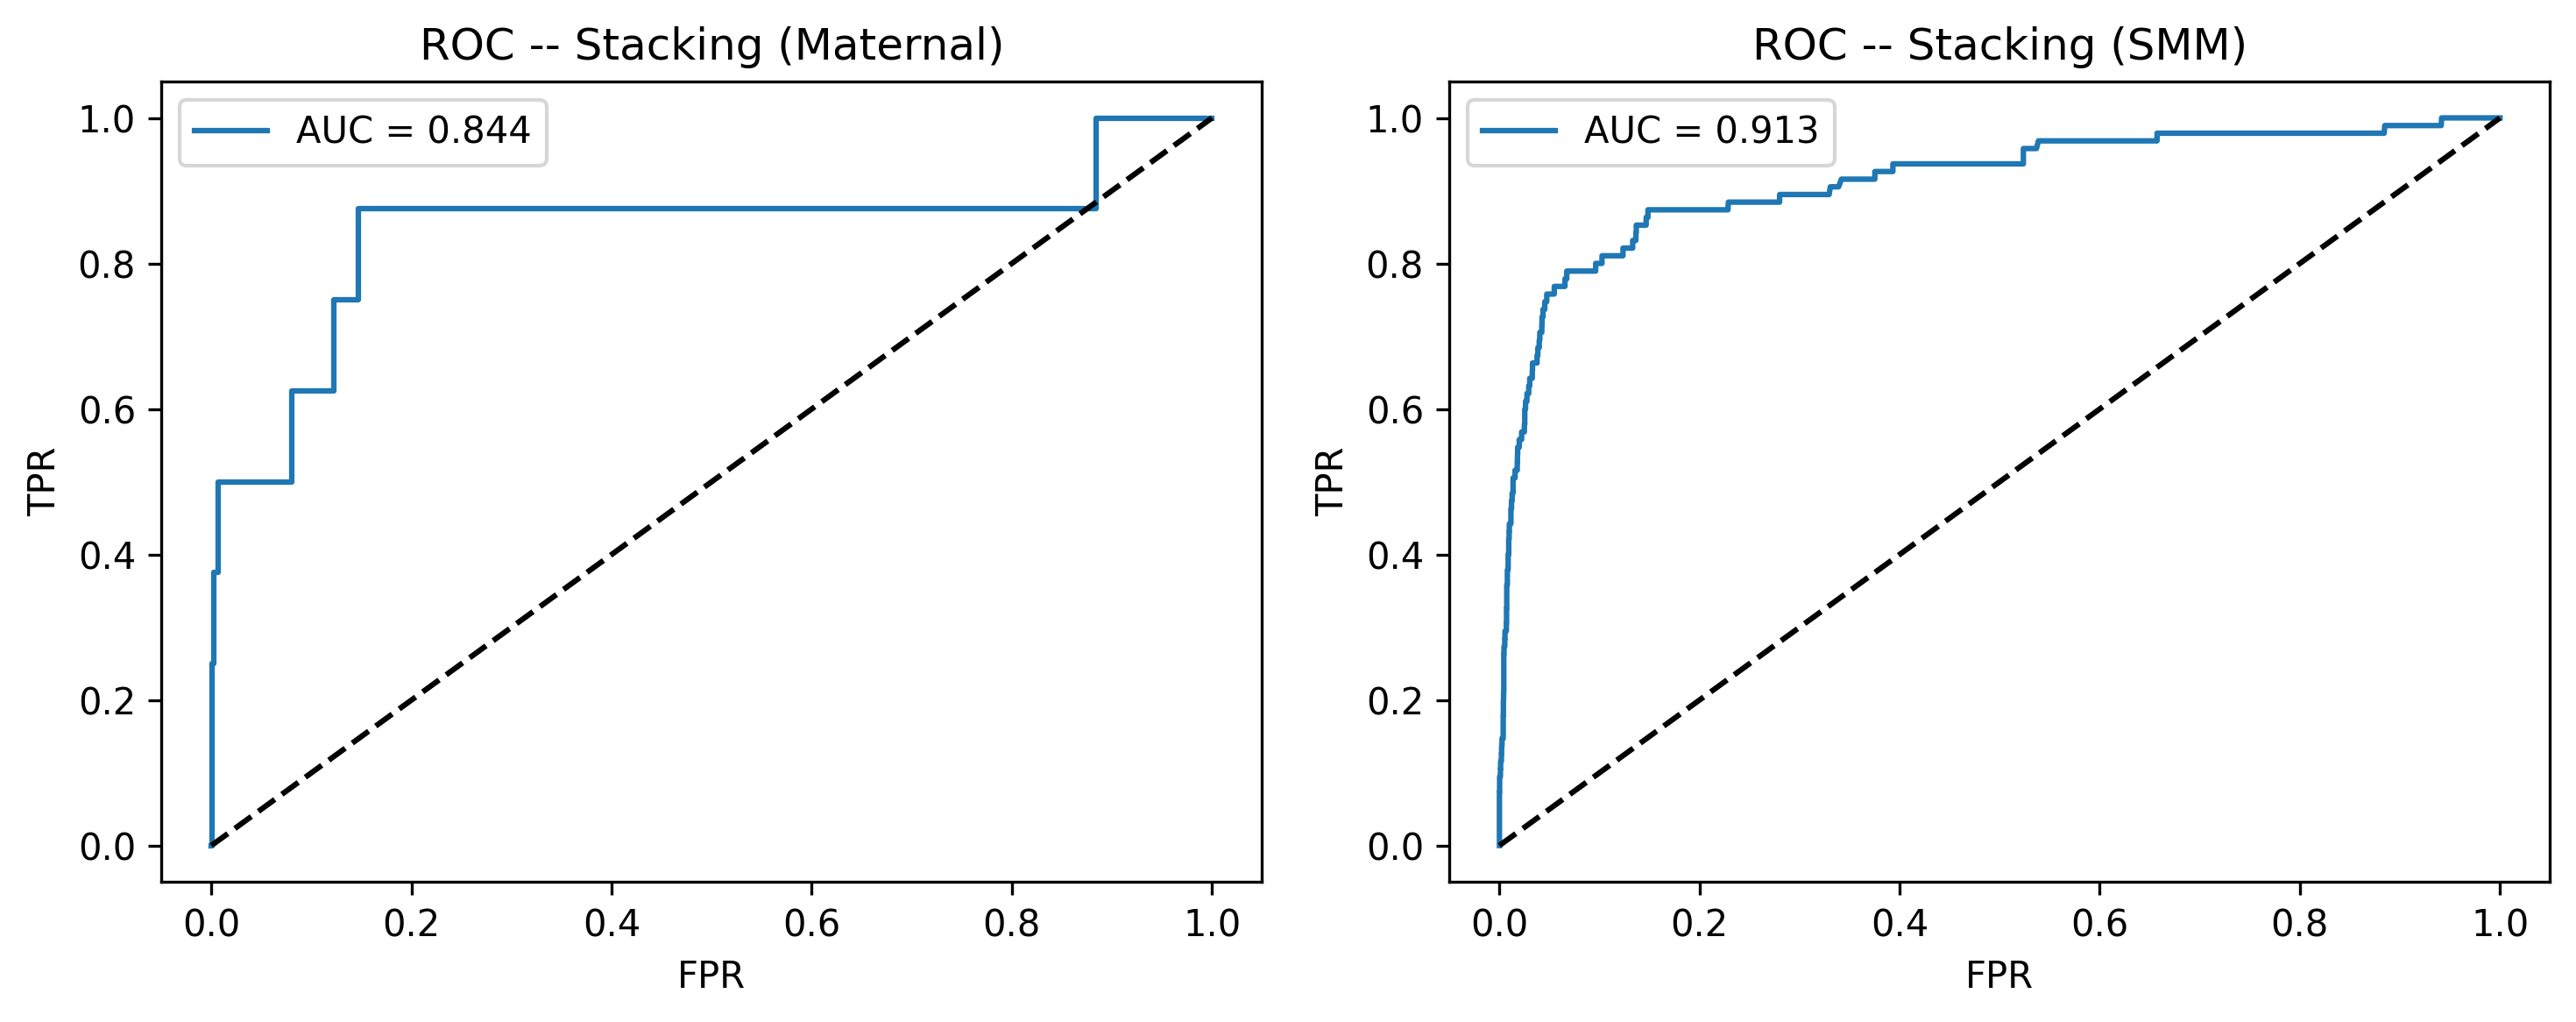
\includegraphics[width=\textwidth]{fig_roc_stacking.png}\\[2mm]
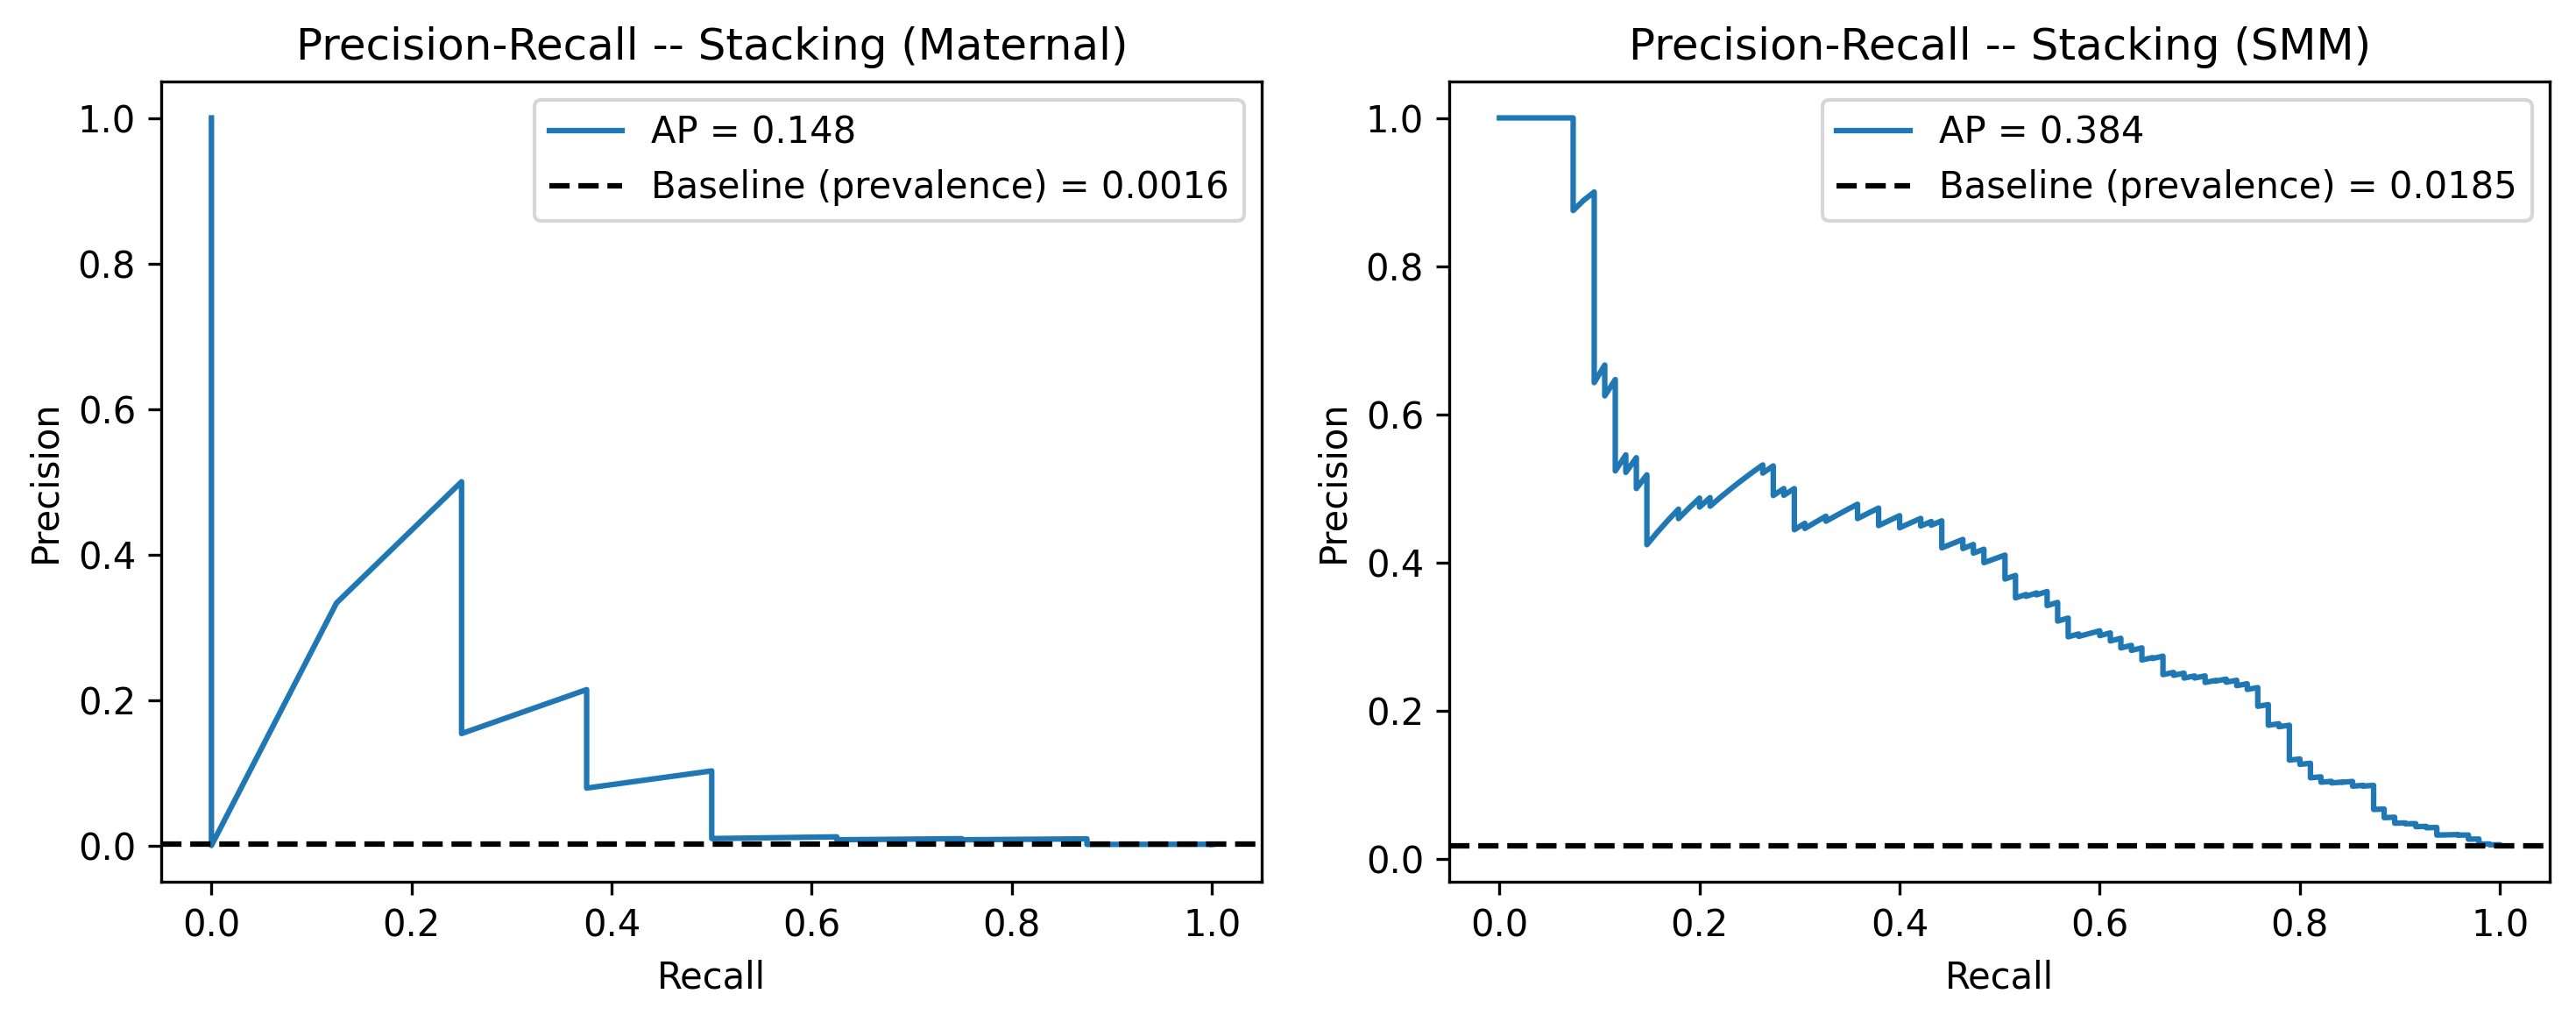
\includegraphics[width=\textwidth]{fig_pr_stacking.png}
\caption{Curvas ROC (arriba) y de precisión--sensibilidad (abajo) del ensamble apilado en
el conjunto de prueba. Izquierda: Modelo~A; derecha: Modelo~B. Las etiquetas de la figura están
en inglés.}\label{fig:rocpr}
\end{figure}

\subsection{Importancia de los predictores}
La Figura~\ref{fig:importance} muestra los 30 predictores más importantes del Random
Forest ajustado para cada modelo. En el Modelo~A, la edad al ingreso ocupó el primer lugar, seguida
del hematocrito, la hemoglobina, los indicadores de grupo diagnóstico \texttt{gdg\_m13}
y \texttt{gdg\_m03}. En el Modelo~B, las primeras posiciones fueron ocupadas por valores de laboratorio:
creatinina, glucosa, bicarbonato, magnesio y hemoglobina. Las importancias basadas en impureza
describen los bosques ajustados y no constituyen evidencia de efectos causales; además, el umbral de
importancia utilizado para la selección de variables se calculó pero no se aplicó, de modo que todos
los predictores se conservaron en cada modelo.

\begin{figure}[H]
\centering
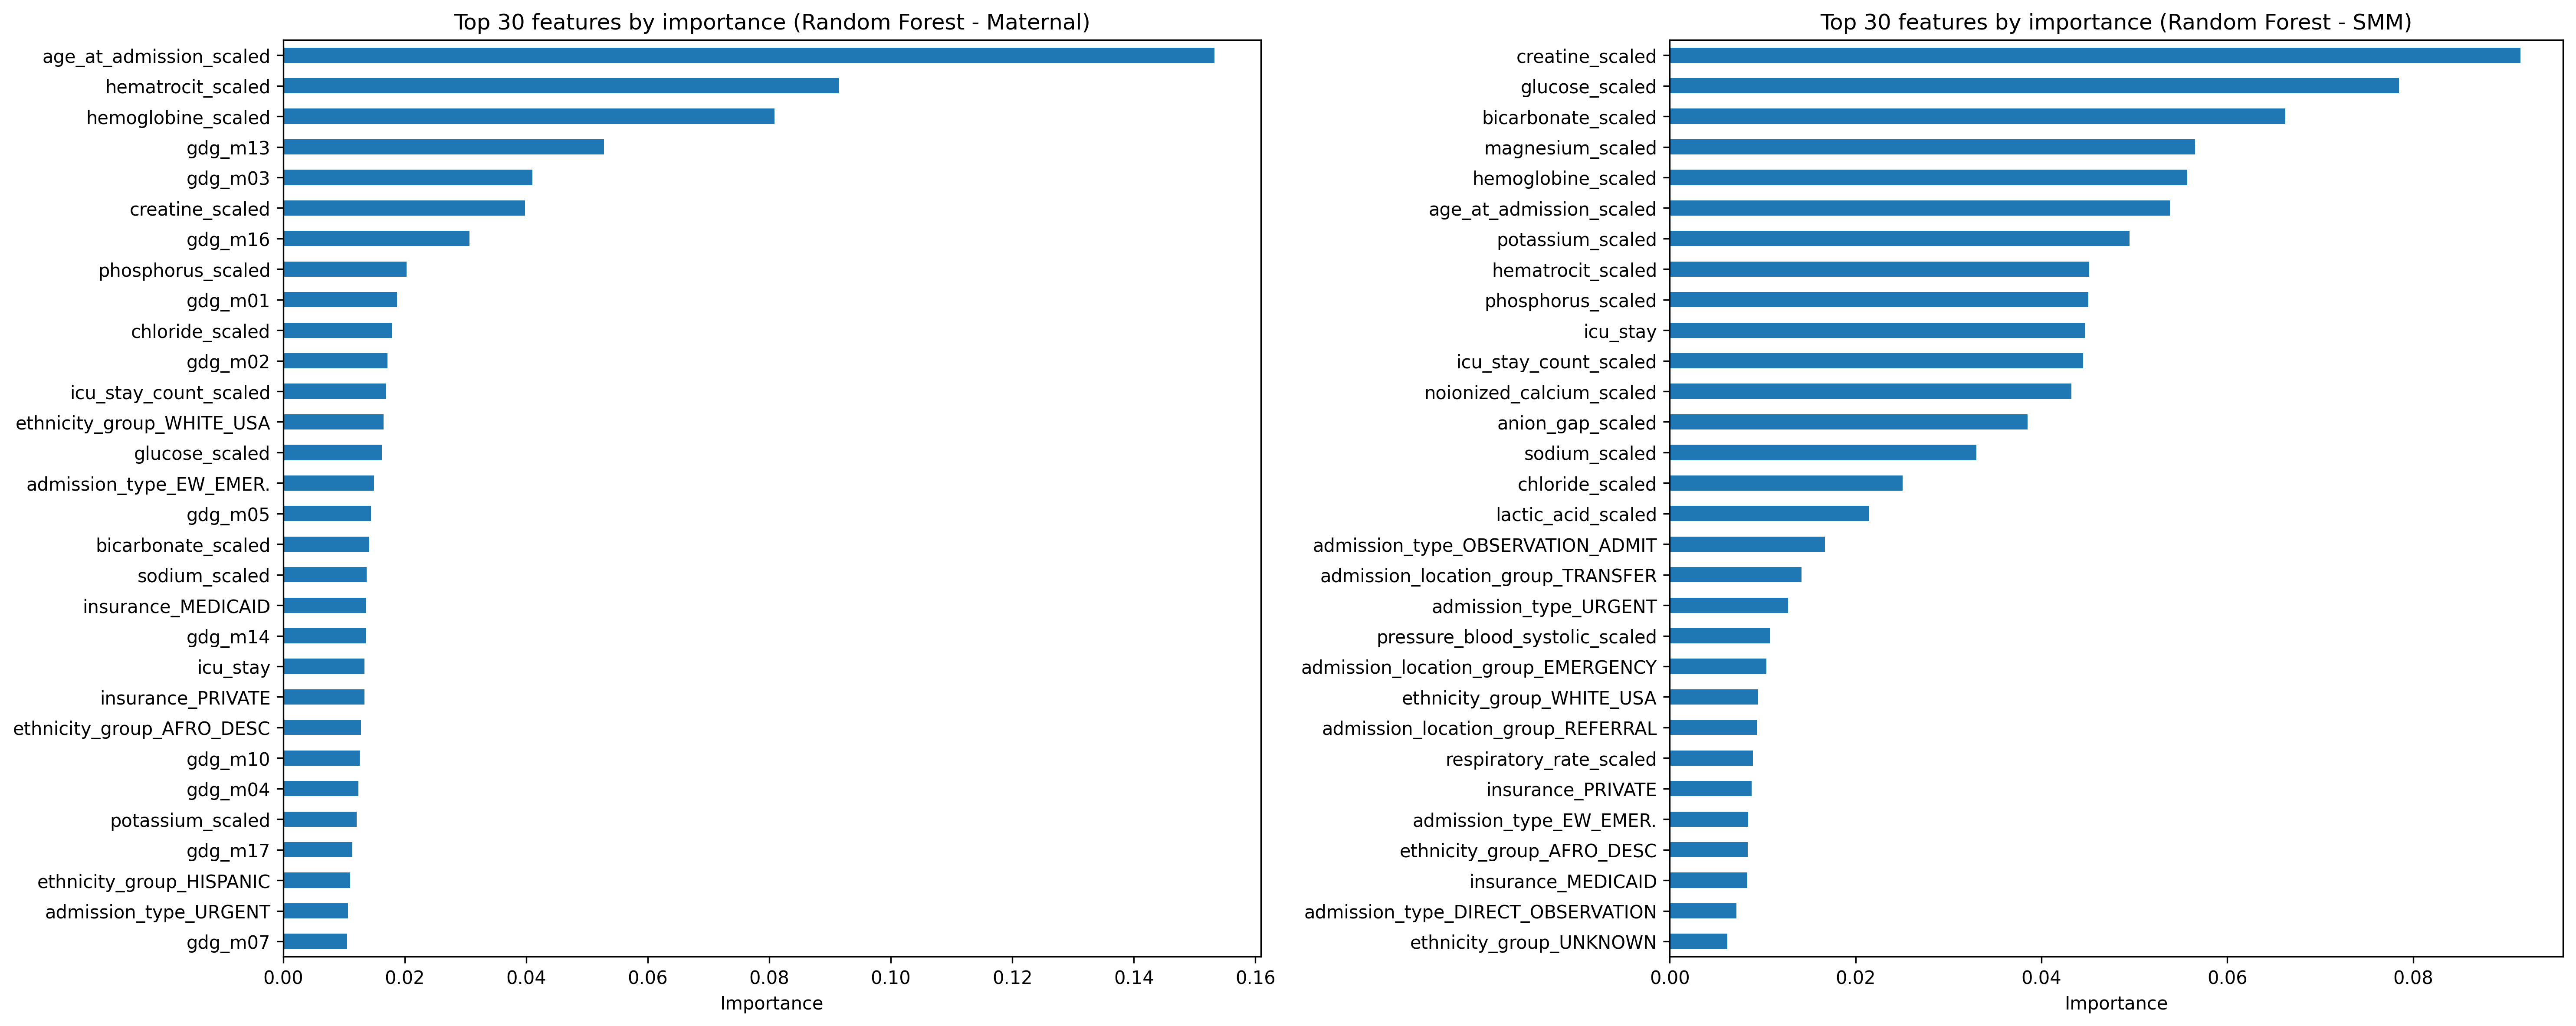
\includegraphics[width=\textwidth]{fig_importance.png}
\caption{Las 30 variables con mayor importancia en Random Forest. Izquierda: Modelo~A; derecha:
Modelo~B. Las etiquetas de la figura están en inglés.}\label{fig:importance}
\end{figure}

\subsection{Análisis adicionales}
\paragraph{Validación cruzada para el Modelo B.}
Sobre toda la cohorte (475 casos de MMG), el mismo protocolo de cinco particiones dio resultados
coherentes con la evaluación en el conjunto de prueba y considerablemente menos dispersos que los del Modelo~A
(Tabla~\ref{tab:cvB}, Figura~\ref{fig:cvB}). El ensamble apilado tuvo el mayor AUC y la mayor AP
(0.904 $\pm$ 0.020 y 0.419 $\pm$ 0.050, unas 23 veces la prevalencia), con XGBoost casi idéntico
(0.901 y 0.413); las desviaciones estándar del AUC entre particiones fueron de 0.017 a 0.029, frente a 0.042 a 0.069
en el Modelo~A. El ensamble apilado también fue el mejor modelo en el conjunto de prueba (AUC 0.913, AP 0.384), aunque las diferencias entre los modelos
superiores son menores que una desviación estándar de la AP. El punto de operación con el umbral por defecto difirió
notablemente entre modelos: el ensamble apilado y XGBoost alcanzaron una sensibilidad de 0.800 y 0.758 a costa de un
F1 bajo (0.234 y 0.264), mientras que Random Forest fue más conservador (sensibilidad 0.467, F1 0.444).

\begin{table}[H]
\caption{Modelo~B: validación cruzada estratificada de cinco particiones (media $\pm$ DE) sobre los
25{,}736 ingresos (475 casos de MMG).\label{tab:cvB}}
\small
\begin{tabularx}{\textwidth}{lCCCC}
\toprule
\textbf{Modelo} & \textbf{AUC} & \textbf{AP} & \textbf{Sensibilidad} & \textbf{F1}\\
\midrule
Random Forest & 0.890 $\pm$ 0.028 & 0.368 $\pm$ 0.037 & 0.467 $\pm$ 0.034 & 0.444 $\pm$ 0.032\\
XGBoost & 0.901 $\pm$ 0.017 & 0.413 $\pm$ 0.038 & 0.758 $\pm$ 0.040 & 0.264 $\pm$ 0.011\\
Extra Trees & 0.885 $\pm$ 0.023 & 0.359 $\pm$ 0.042 & 0.560 $\pm$ 0.041 & 0.362 $\pm$ 0.035\\
Regresión logística & 0.876 $\pm$ 0.029 & 0.342 $\pm$ 0.048 & 0.749 $\pm$ 0.074 & 0.233 $\pm$ 0.018\\
Apilamiento & \textbf{0.904} $\pm$ 0.020 & \textbf{0.419} $\pm$ 0.050 & 0.800 $\pm$ 0.040 & 0.234 $\pm$ 0.013\\
\bottomrule
\end{tabularx}
\end{table}
\unskip
\begin{figure}[H]
\centering
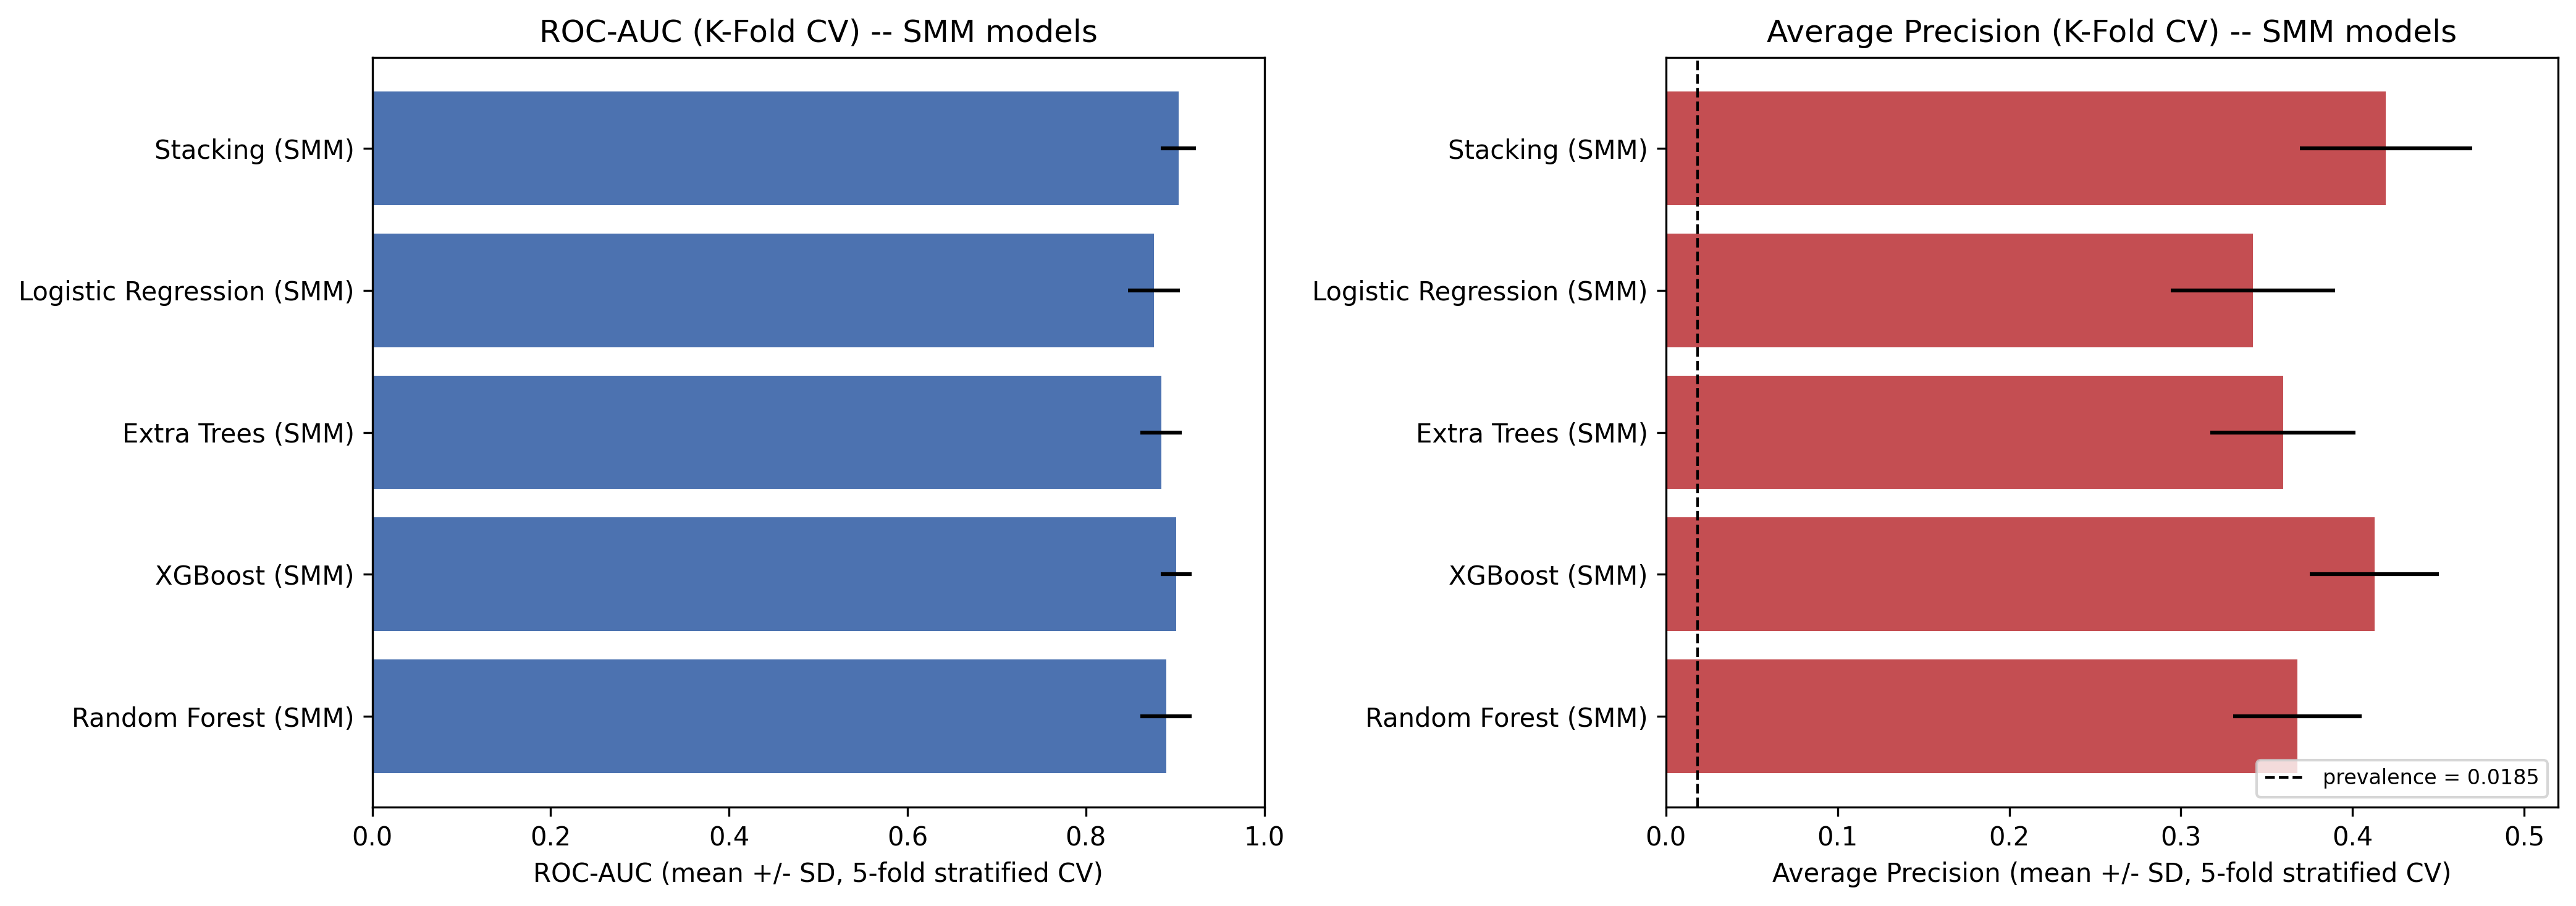
\includegraphics[width=\textwidth]{fig_cv_B.png}
\caption{Modelo~B: AUC y AP con validación cruzada de cinco particiones (media y desviación estándar); la línea discontinua es la prevalencia. Las etiquetas de la figura están en inglés.}\label{fig:cvB}
\end{figure}

\paragraph{Análisis de sensibilidad con sobremuestreo (Modelo B).}
SMOTE tampoco mejoró las métricas basadas en precisión del Modelo~B (Tabla~\ref{tab:smoteB}, Figura~\ref{fig:smoteB}).
La AP del ensamble apilado pasó de 0.419 a 0.406 y la de XGBoost de 0.413 a 0.350, mientras que
el AUC del ensamble apilado pasó de 0.904 a 0.896. Solo Random Forest (AUC de 0.890 a 0.899) y la regresión logística (AP de 0.342 a
0.357) mostraron pequeñas mejoras. SMOTE desplazó en cambio el punto de operación: la sensibilidad de XGBoost subió de
0.758 a 0.964, pero con un F1 de 0.047, es decir, se marcó casi la totalidad de los ingresos, mientras que la sensibilidad del ensamble apilado cayó de 0.800 a
0.636. Como en el Modelo~A, se mantuvo la ponderación de clases como opción por defecto.

\begin{table}[H]
\caption{Modelo~B: efecto de SMOTE (estrategia de muestreo 0.2) sobre el AUC, la AP y la sensibilidad con validación cruzada de cinco
particiones (valores medios).\label{tab:smoteB}}
\small
\begin{tabularx}{\textwidth}{lCCCCCC}
\toprule
 & \multicolumn{2}{c}{\textbf{AUC}} & \multicolumn{2}{c}{\textbf{AP}} & \multicolumn{2}{c}{\textbf{Sensibilidad}}\\
\cmidrule(lr){2-3}\cmidrule(lr){4-5}\cmidrule(lr){6-7}
\textbf{Modelo} & Pesos & SMOTE & Pesos & SMOTE & Pesos & SMOTE\\
\midrule
Random Forest & 0.890 & 0.899 & 0.368 & 0.366 & 0.467 & 0.539\\
XGBoost & 0.901 & 0.892 & 0.413 & 0.350 & 0.758 & 0.964\\
Extra Trees & 0.885 & 0.875 & 0.359 & 0.349 & 0.560 & 0.535\\
Regresión logística & 0.876 & 0.825 & 0.342 & 0.357 & 0.749 & 0.554\\
Apilamiento & 0.904 & 0.896 & 0.419 & 0.406 & 0.800 & 0.636\\
\bottomrule
\end{tabularx}
\end{table}
\unskip
\begin{figure}[H]
\centering
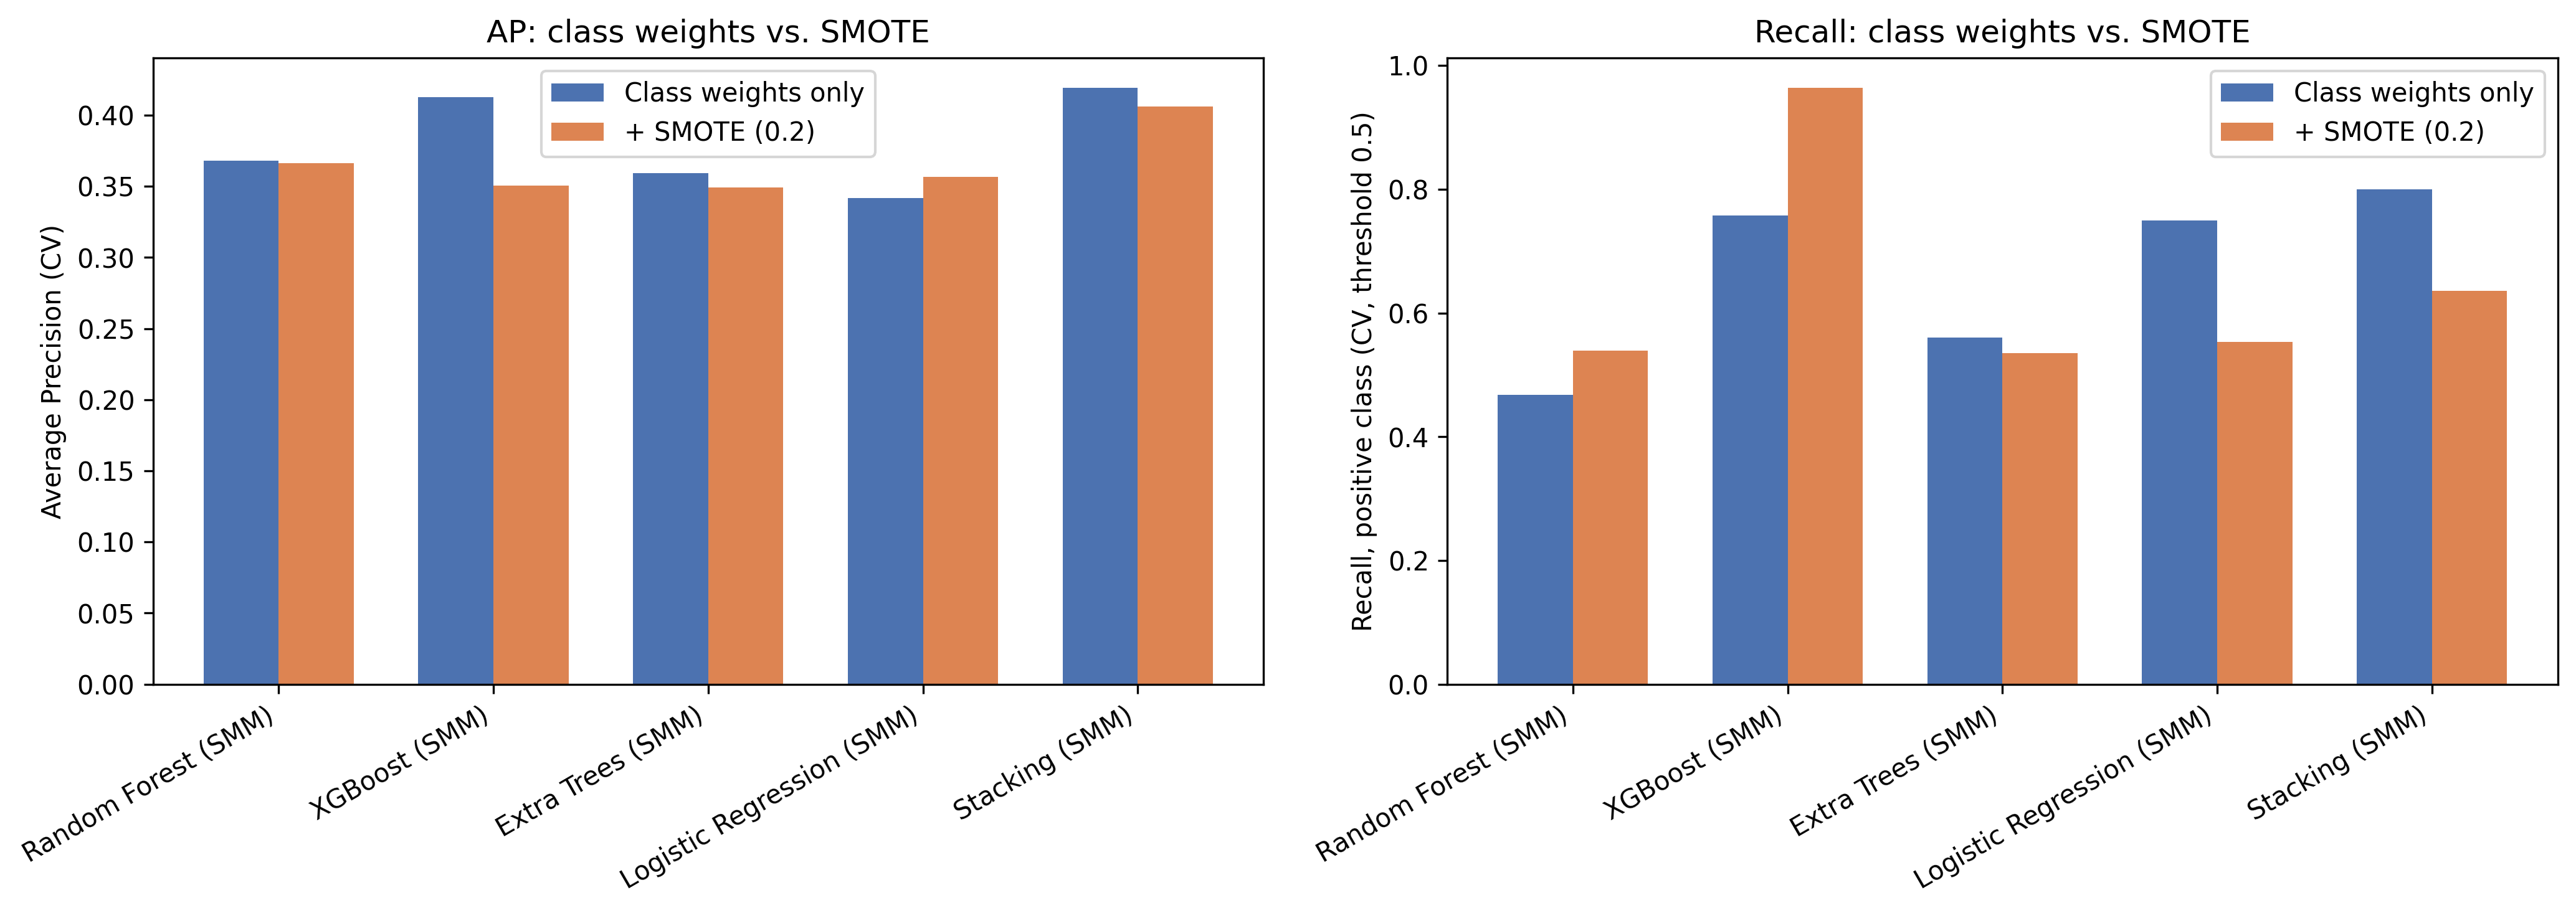
\includegraphics[width=\textwidth]{fig_smote_B.png}
\caption{Modelo~B: ponderación de clases frente a SMOTE con validación cruzada de cinco particiones (izquierda: AP; derecha: sensibilidad con umbral 0.5). Las etiquetas de la figura están en inglés.}\label{fig:smoteB}
\end{figure}

\paragraph{Modelo A sin grupos diagnósticos.}
La Tabla~\ref{tab:nogdg} compara el desempeño con validación cruzada del Modelo~A con y sin los
26 indicadores de grupos diagnósticos. Retirarlos redujo el AUC de todos los modelos
(apilamiento de 0.857 a 0.725, RF de 0.809 a 0.700, XGB de 0.817 a 0.690, ET de 0.831 a 0.768, LR de 0.758 a
0.635) y llevó la AP a la baja en cuatro de los cinco modelos (a 0.007--0.039; apilamiento de 0.156 a 0.013, frente a una
prevalencia de 0.0016); solo LR aumentó (de 0.049 a 0.061, con una desviación estándar de 0.062). En el conjunto de prueba, el ensamble apilado pasó de un AUC de 0.844 y una AP de
0.148 a 0.731 y 0.020 (ocho positivos; solo ilustrativo). Por tanto, la mayor parte de la señal discriminativa del Modelo~A
proviene de los grupos diagnósticos, que se derivan de los códigos CIE del propio ingreso.

\begin{table}[H]
\caption{Modelo~A: AUC y AP con validación cruzada con y sin los indicadores de grupos diagnósticos
(hiperparámetros conservados; valores medios).\label{tab:nogdg}}
\small
\begin{tabularx}{\textwidth}{lCCCC}
\toprule
 & \multicolumn{2}{c}{\textbf{AUC}} & \multicolumn{2}{c}{\textbf{AP}}\\
\cmidrule(lr){2-3}\cmidrule(lr){4-5}
\textbf{Modelo} & Con & Sin & Con & Sin\\
\midrule
Random Forest & 0.809 & 0.700 & 0.115 & 0.007\\
XGBoost & 0.817 & 0.690 & 0.165 & 0.039\\
Extra Trees & 0.831 & 0.768 & 0.190 & 0.021\\
Regresión logística & 0.758 & 0.635 & 0.049 & 0.061\\
Apilamiento & 0.857 & 0.725 & 0.156 & 0.013\\
\bottomrule
\end{tabularx}
\end{table}

\paragraph{Calibración y estratificación del riesgo del Modelo A.}
Con las probabilidades fuera de partición del ensamble apilado sobre toda la cohorte (41 muertes), el AUC fue 0.842
(intervalo de confianza \emph{bootstrap} del 95\%: 0.771--0.914) y la AP fue 0.123 (0.036--0.251). Como es esperable tras la
ponderación de clases, las probabilidades predichas fueron muy superiores a la frecuencia observada: la
probabilidad media predicha fue 0.379 frente a una prevalencia observada de 0.0016 (razón 237.8), el puntaje de Brier fue 0.162
(0.0016 para un modelo que siempre predice la prevalencia; habilidad de Brier $-100.9$) y la curva de confiabilidad
quedó por debajo de la diagonal en todo su rango (Figura~\ref{fig:calibA}). Las medidas basadas en el orden no dependen de la calibración
(Tabla~\ref{tab:topxA}). Marcar el 5\% superior de los ingresos (1{,}287) capturó 18 de las 41 muertes (sensibilidad 0.439,
intervalo de confianza del 95\%: 0.286--0.615; valor predictivo positivo 0.014, 0.008--0.021; \emph{lift} 8.8). Con
bandas de riesgo basadas en percentiles, la mortalidad observada fue 0.06\% en la banda baja (por debajo del percentil 80; 12 muertes
entre 20{,}588 ingresos), 0.28\% en la banda moderada (percentil 80 a 95; 11 de 3{,}861) y 1.40\% en la banda alta
(5\% superior; 18 de 1{,}287), un gradiente de unas 24 veces entre la banda alta y la baja. En el conjunto de prueba, 4 de las 8
muertes cayeron en la banda alta, 3 en la moderada y 1 en la baja.

\begin{table}[H]
\caption{Modelo~A: tabla de ``marcar el $x$\% superior'' a partir de las predicciones fuera de partición del ensamble apilado
(41 muertes entre 25{,}736 ingresos).\label{tab:topxA}}
\small
\setlength{\tabcolsep}{3pt}
\begin{tabularx}{\textwidth}{lCCCCC}
\toprule
\textbf{$x$\% superior marcado} & \textbf{Ingresos} & \textbf{Muertes capturadas} & \textbf{Sensibilidad} & \textbf{VPP} & \textbf{\emph{Lift}}\\
\midrule
0.5\% & 129 & 11 & 0.268 & 0.0853 & 53.5\\
1\% & 257 & 13 & 0.317 & 0.0506 & 31.8\\
2\% & 515 & 14 & 0.341 & 0.0272 & 17.1\\
5\% & 1{,}287 & 18 & 0.439 & 0.0140 & 8.8\\
10\% & 2{,}574 & 22 & 0.537 & 0.0085 & 5.4\\
20\% & 5{,}147 & 29 & 0.707 & 0.0056 & 3.5\\
\bottomrule
\end{tabularx}
\end{table}
\unskip
\begin{figure}[H]
\centering
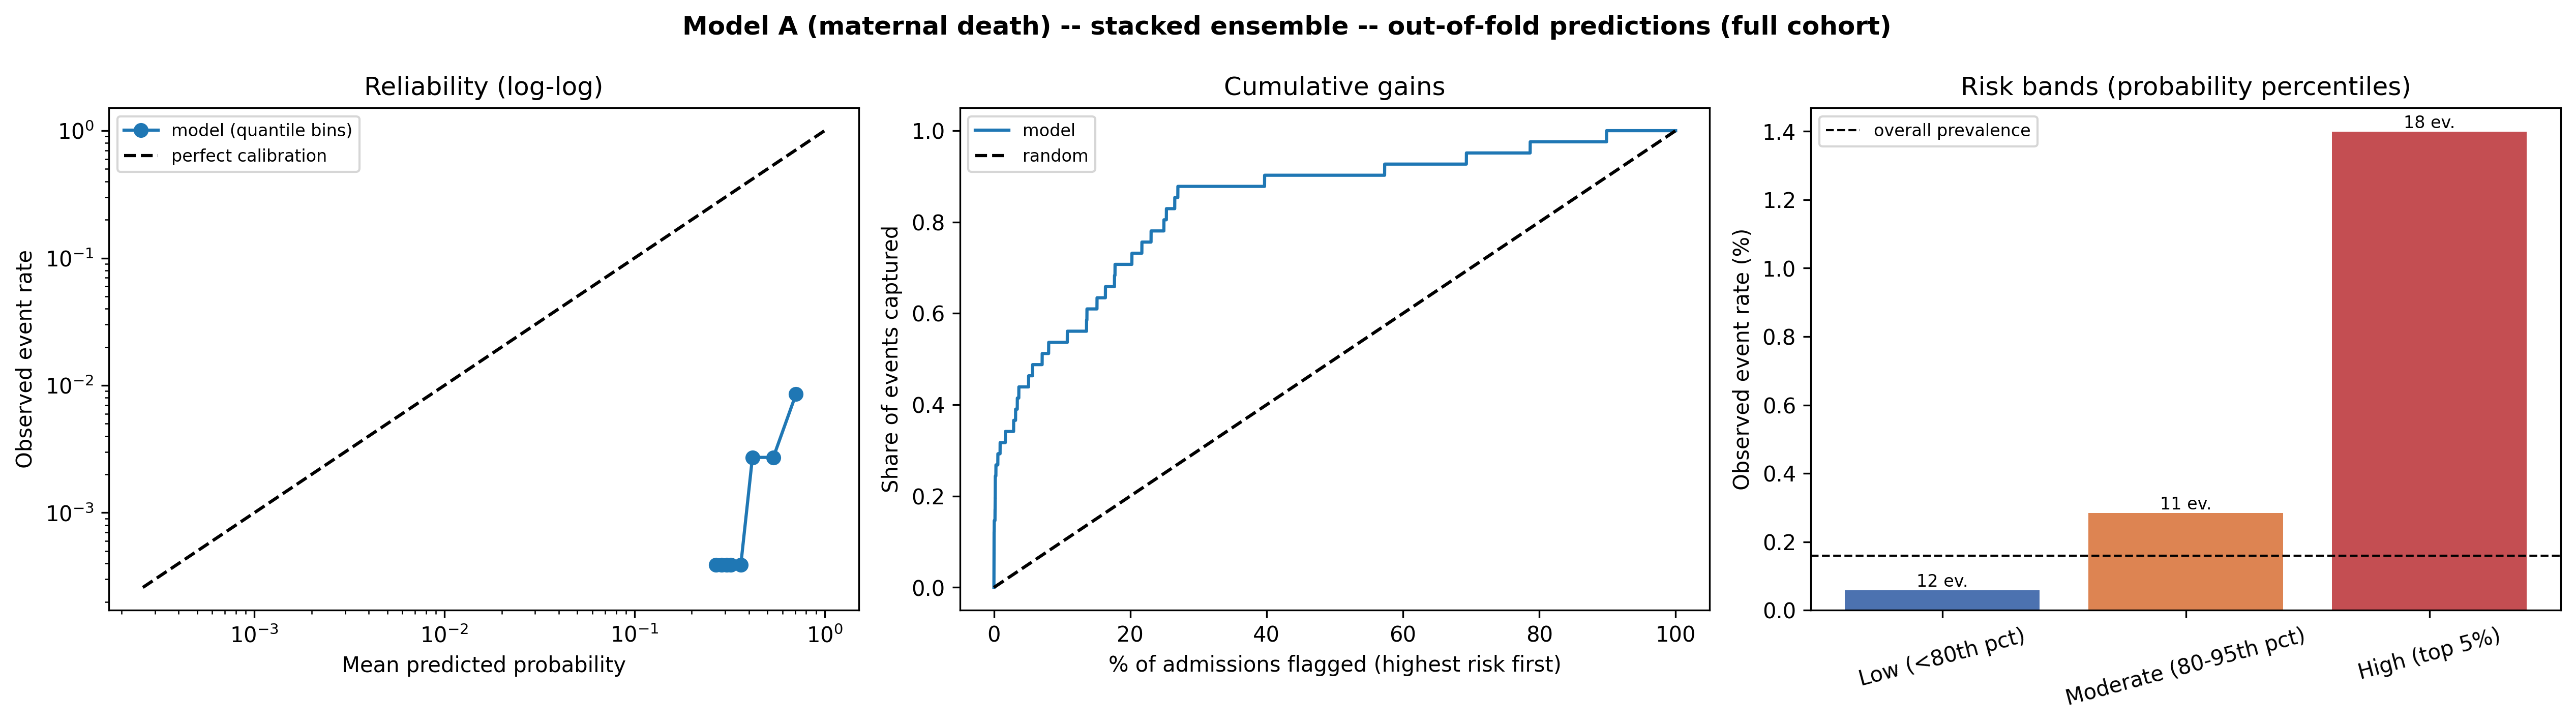
\includegraphics[width=\textwidth]{fig_calib_A_oof.png}
\caption{Modelo~A, ensamble apilado, predicciones fuera de partición sobre toda la cohorte: curva de confiabilidad
(escala log--log), ganancias acumuladas y mortalidad observada por banda de riesgo. Las etiquetas de la figura están en inglés.}\label{fig:calibA}
\end{figure}

\paragraph{Calibración y estratificación del riesgo del Modelo B.}
Las probabilidades fuera de partición del ensamble apilado sobre toda la cohorte (475 casos de MMG) dieron un AUC de 0.902
(intervalo de confianza \emph{bootstrap} del 95\%: 0.884--0.920) y una AP de 0.396 (0.349--0.454). Las probabilidades fueron
de nuevo mucho mayores que la frecuencia observada: la probabilidad media predicha fue 0.249 frente a una prevalencia de 0.0185
(razón 13.5), el puntaje de Brier fue 0.092 (0.018 para un modelo que siempre predice la prevalencia; habilidad de Brier $-4.10$)
y la curva de confiabilidad quedó por debajo de la diagonal (Figura~\ref{fig:calibB}). El conjunto de prueba mostró el mismo patrón (probabilidad media
predicha 0.252, razón 13.6; puntaje de Brier 0.093). Por tanto, las probabilidades brutas deben usarse para ordenar ingresos y no como riesgos absolutos (véase la recalibración a continuación).
En términos de ordenamiento (Tabla~\ref{tab:topxB}), marcar el 5\% superior de los ingresos (1{,}287) capturó 324 de los 475 casos de MMG
(sensibilidad 0.682, intervalo de confianza \emph{bootstrap} del 95\%: 0.643--0.719; valor predictivo positivo 0.252, 0.226--0.277; \emph{lift} 13.6),
y marcar el 1\% superior (257) ya capturó 151 casos con un valor predictivo positivo de 0.588. Con bandas de riesgo basadas en percentiles,
la tasa observada de MMG fue 0.34\% en la banda baja (70 casos entre 20{,}588 ingresos), 2.10\% en la banda moderada
(81 de 3{,}861) y 25.2\% en la banda alta (324 de 1{,}287), un gradiente de unas 74 veces entre la banda alta y la baja; la
banda alta contuvo el 68\% de todos los casos y la baja el 15\%. En el conjunto de prueba, 64 de los 95 casos cayeron en la banda alta (tasa observada 24.8\%),
19 en la moderada (2.5\%) y 12 en la baja (0.29\%); la sensibilidad y el valor predictivo positivo en el 5\% superior fueron 0.674 (0.589--0.780) y 0.249 (0.195--0.309).
Se usaron bandas basadas en percentiles porque los puntos de corte de probabilidad (0.27 y 0.80 para las bandas moderada y alta) son específicos de este
modelo y no tienen significado como riesgos absolutos.

\begin{table}[H]
\caption{Modelo~B: tabla de ``marcar el $x$\% superior'' a partir de las predicciones fuera de partición del ensamble apilado
(475 casos de MMG entre 25{,}736 ingresos).\label{tab:topxB}}
\small
\setlength{\tabcolsep}{3pt}
\begin{tabularx}{\textwidth}{lCCCCC}
\toprule
\textbf{$x$\% superior marcado} & \textbf{Ingresos} & \textbf{Casos capturados} & \textbf{Sensibilidad} & \textbf{VPP} & \textbf{\emph{Lift}}\\
\midrule
0.5\% & 129 & 79 & 0.166 & 0.612 & 33.2\\
1\% & 257 & 151 & 0.318 & 0.588 & 31.8\\
2\% & 515 & 238 & 0.501 & 0.462 & 25.0\\
5\% & 1{,}287 & 324 & 0.682 & 0.252 & 13.6\\
10\% & 2{,}574 & 372 & 0.783 & 0.145 & 7.8\\
20\% & 5{,}147 & 405 & 0.853 & 0.079 & 4.3\\
\bottomrule
\end{tabularx}
\end{table}
\unskip
\begin{figure}[H]
\centering
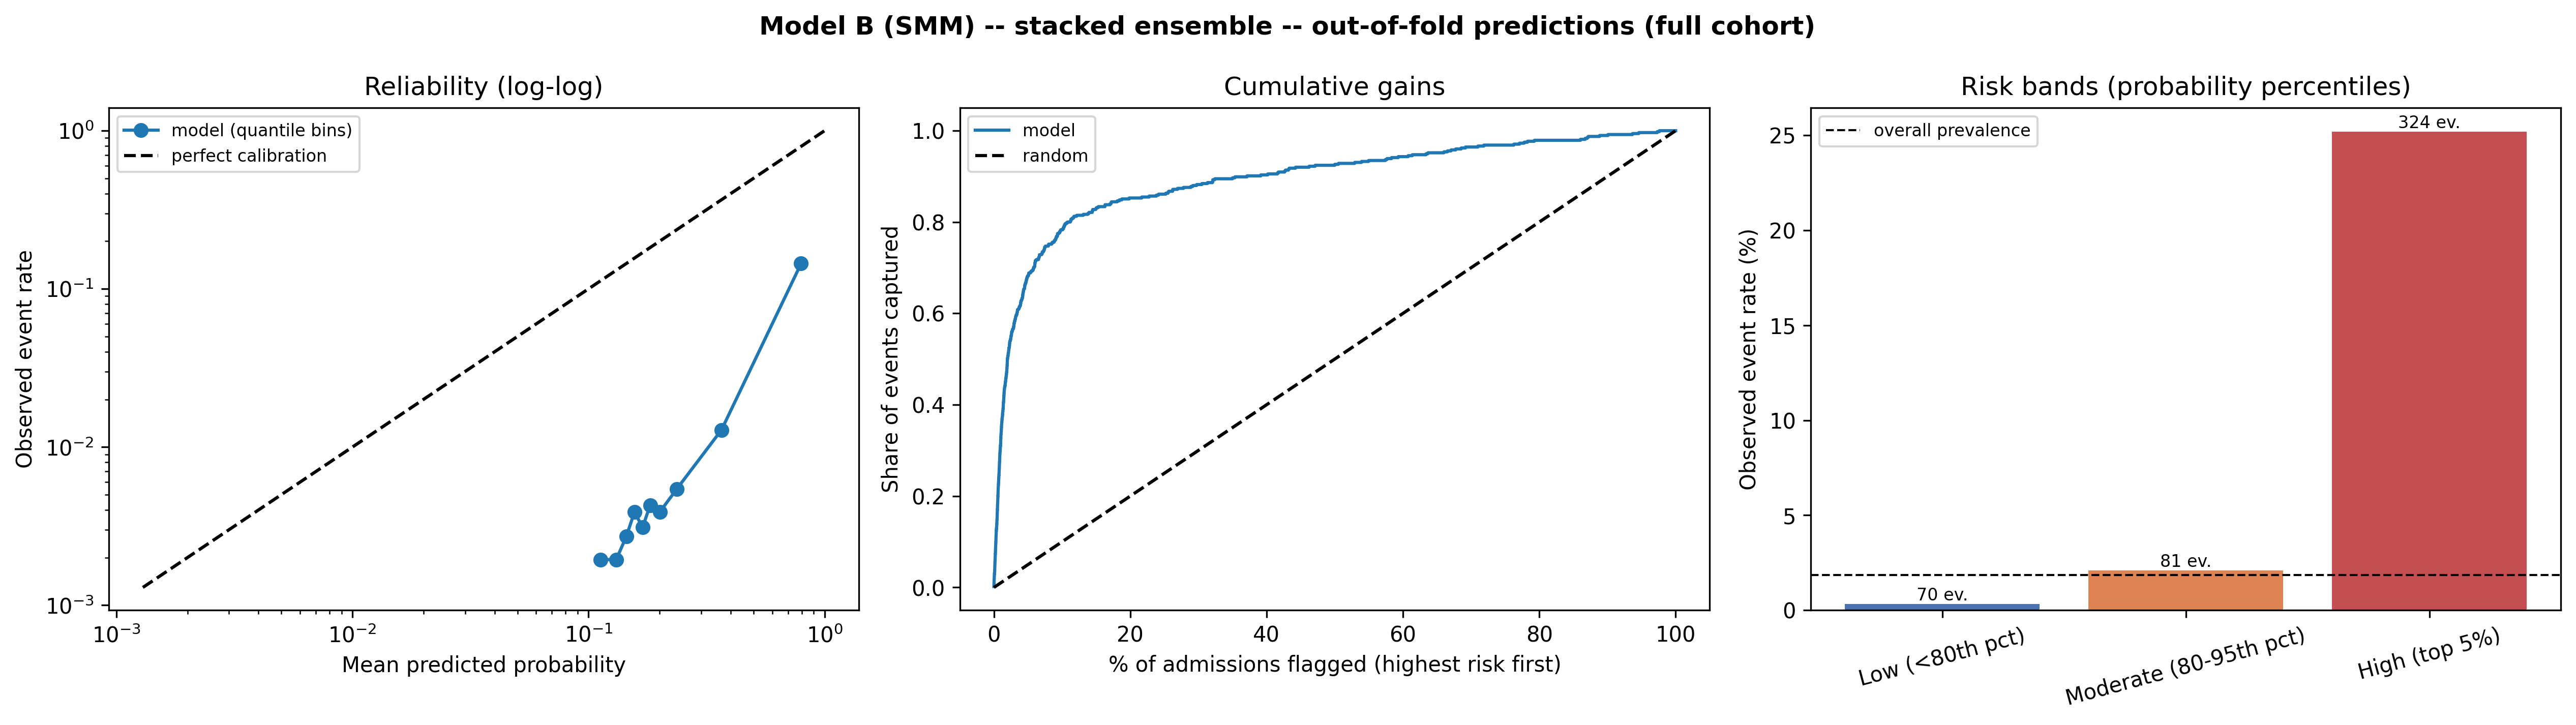
\includegraphics[width=\textwidth]{fig_calib_B_oof.png}
\caption{Modelo~B, ensamble apilado, predicciones fuera de partición sobre toda la cohorte: curva de confiabilidad
(escala log--log), ganancias acumuladas y tasa observada de MMG por banda de riesgo. Las etiquetas de la figura están en inglés.}\label{fig:calibB}
\end{figure}

\paragraph{Recalibración.}
Dado que la ponderación de clases infla las probabilidades predichas, se recalibraron a posteriori las probabilidades fuera de partición del ensamble
apilado (Tabla~\ref{tab:recal}, Figura~\ref{fig:recal}). En el Modelo~B, el escalamiento de Platt llevó la razón entre la probabilidad media predicha y la prevalencia
de 13.5 a 1.00, redujo el ECE de 0.231 a 0.0009, dejó la pendiente de calibración en 1.00 y cambió la habilidad de Brier de
$-4.10$ a 0.26 (puntaje de Brier de 0.0925 a 0.0134), con una discriminación prácticamente sin cambios (AUC de 0.902 a 0.901; AP de 0.396 a 0.394).
La regresión isotónica dio una calibración similar (habilidad de Brier 0.256) pero una discriminación algo menor (AUC 0.895; AP 0.370), como es esperable de una
función escalonada que genera empates entre probabilidades. En el Modelo~A, el escalamiento de Platt también eliminó la mayor parte de la descalibración (razón de 237.8 a 1.01; ECE de 0.377 a 0.0006), pero la habilidad
de Brier solo alcanzó 0.064, porque el puntaje de Brier (0.0015) es apenas inferior al de un modelo que siempre predice la prevalencia (0.0016), y el AUC bajó de 0.842 a 0.836
(AP de 0.123 a 0.115). La regresión isotónica fue menos estable en el Modelo~A (pendiente de calibración 0.73; AUC 0.805; AP 0.098), pues 41 eventos no sustentan un mapa de calibración flexible.
La recalibración convierte entonces las puntuaciones del Modelo~B en estimaciones de riesgo utilizables en esta cohorte, mientras que en el Modelo~A las deja calibradas
pero apenas más informativas que la prevalencia. Los mapas de calibración se estimaron mediante validación cruzada repetida dentro de la misma cohorte y
requieren validación externa.

\begin{table}[H]
\caption{Recalibración a posteriori de las probabilidades fuera de partición del ensamble apilado (media de 20 repeticiones de validación cruzada de cinco particiones): puntaje de Brier y
habilidad de Brier (relativa a un modelo que predice la prevalencia), razón entre la probabilidad media predicha y la prevalencia, error de calibración esperado (ECE, diez intervalos por cuantiles),
pendiente de calibración, AUC y AP.\label{tab:recal}}
\scriptsize
\setlength{\tabcolsep}{3pt}
\begin{tabularx}{\textwidth}{llCCCCCCC}
\toprule
\textbf{Modelo} & \textbf{Probabilidades} & \textbf{Brier} & \textbf{Habilidad} & \textbf{Razón} & \textbf{ECE} & \textbf{Pendiente} & \textbf{AUC} & \textbf{AP}\\
\midrule
A (mortalidad) & Brutas (ponderadas) & 0.1621 & $-100.9$ & 237.8 & 0.377 & 1.08 & 0.842 & 0.123\\
 & Platt & 0.0015 & 0.064 & 1.01 & 0.0006 & 0.98 & 0.836 & 0.115\\
 & Isotónica & 0.0015 & 0.055 & 1.01 & 0.0006 & 0.73 & 0.805 & 0.098\\
\midrule
B (MMG) & Brutas (ponderadas) & 0.0925 & $-4.10$ & 13.5 & 0.231 & 1.04 & 0.902 & 0.396\\
 & Platt & 0.0134 & 0.260 & 1.00 & 0.0009 & 1.00 & 0.901 & 0.394\\
 & Isotónica & 0.0135 & 0.256 & 1.00 & 0.0011 & 0.97 & 0.895 & 0.370\\
\bottomrule
\end{tabularx}
\end{table}
\unskip
\begin{figure}[H]
\centering
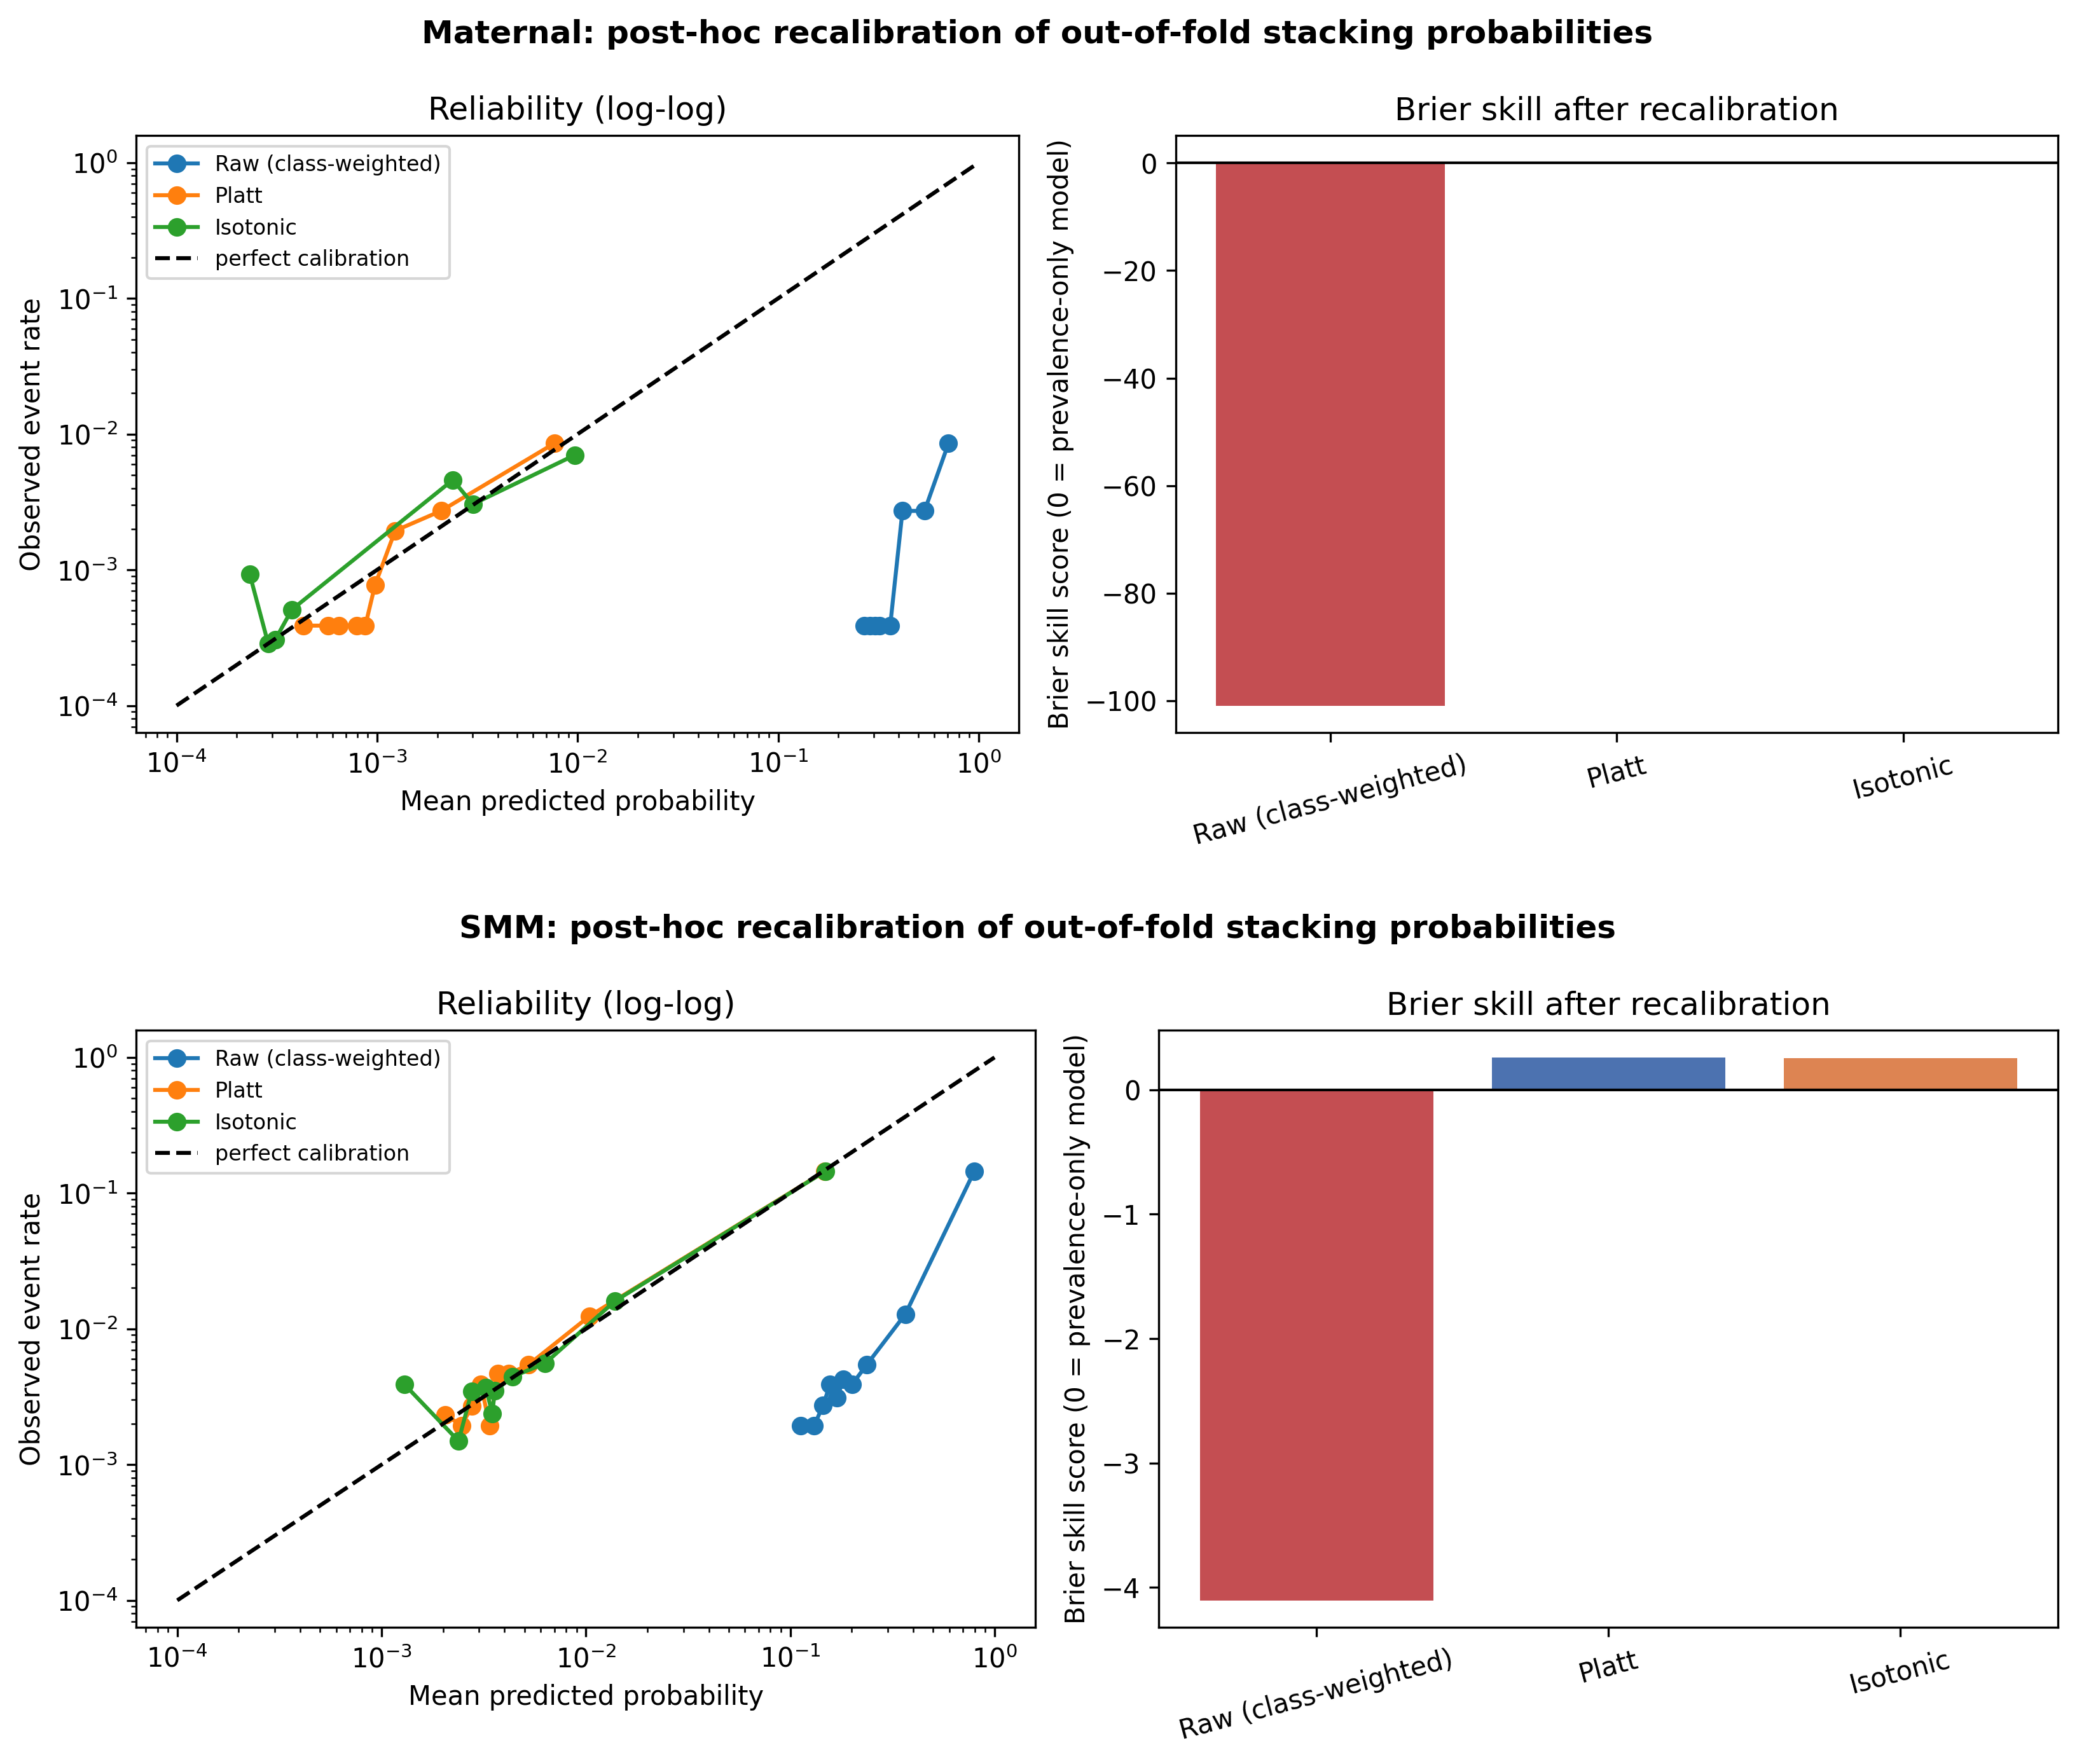
\includegraphics[width=0.85\textwidth]{fig_recal.png}
\caption{Recalibración a posteriori de las probabilidades fuera de partición del ensamble apilado: curvas de confiabilidad (escala log--log) y habilidad de Brier
para el Modelo~A (arriba) y el Modelo~B (abajo). Las etiquetas de la figura están en inglés.}\label{fig:recal}
\end{figure}

\paragraph{Explicabilidad y auditoría por subgrupos.}
Los valores SHAP absolutos medios del aprendiz base XGBoost en el conjunto de prueba fueron mayores para creatinina (0.28),
glucosa (0.24), estancia en UCI (0.24), bicarbonato (0.18), ácido láctico (0.16), magnesio (0.14), edad (0.13) y
hemoglobina (0.13), seguidos de hematocrito, los tipos de ingreso por observación y urgente, y los ingresos por traslado (0.08--0.09)
(Figura~\ref{fig:shap}). El orden concuerda con las importancias de Random Forest (valores de laboratorio renales y metabólicos en los primeros lugares) y añade la estancia en UCI y
el ácido láctico. Son descripciones del modelo ajustado y no efectos causales; además, la estancia en UCI y el lactato pueden seguir
al evento mórbido en lugar de precederlo, por lo que su peso debe leerse con la salvedad sobre la temporalidad que se discute más adelante.

\begin{figure}[H]
\centering
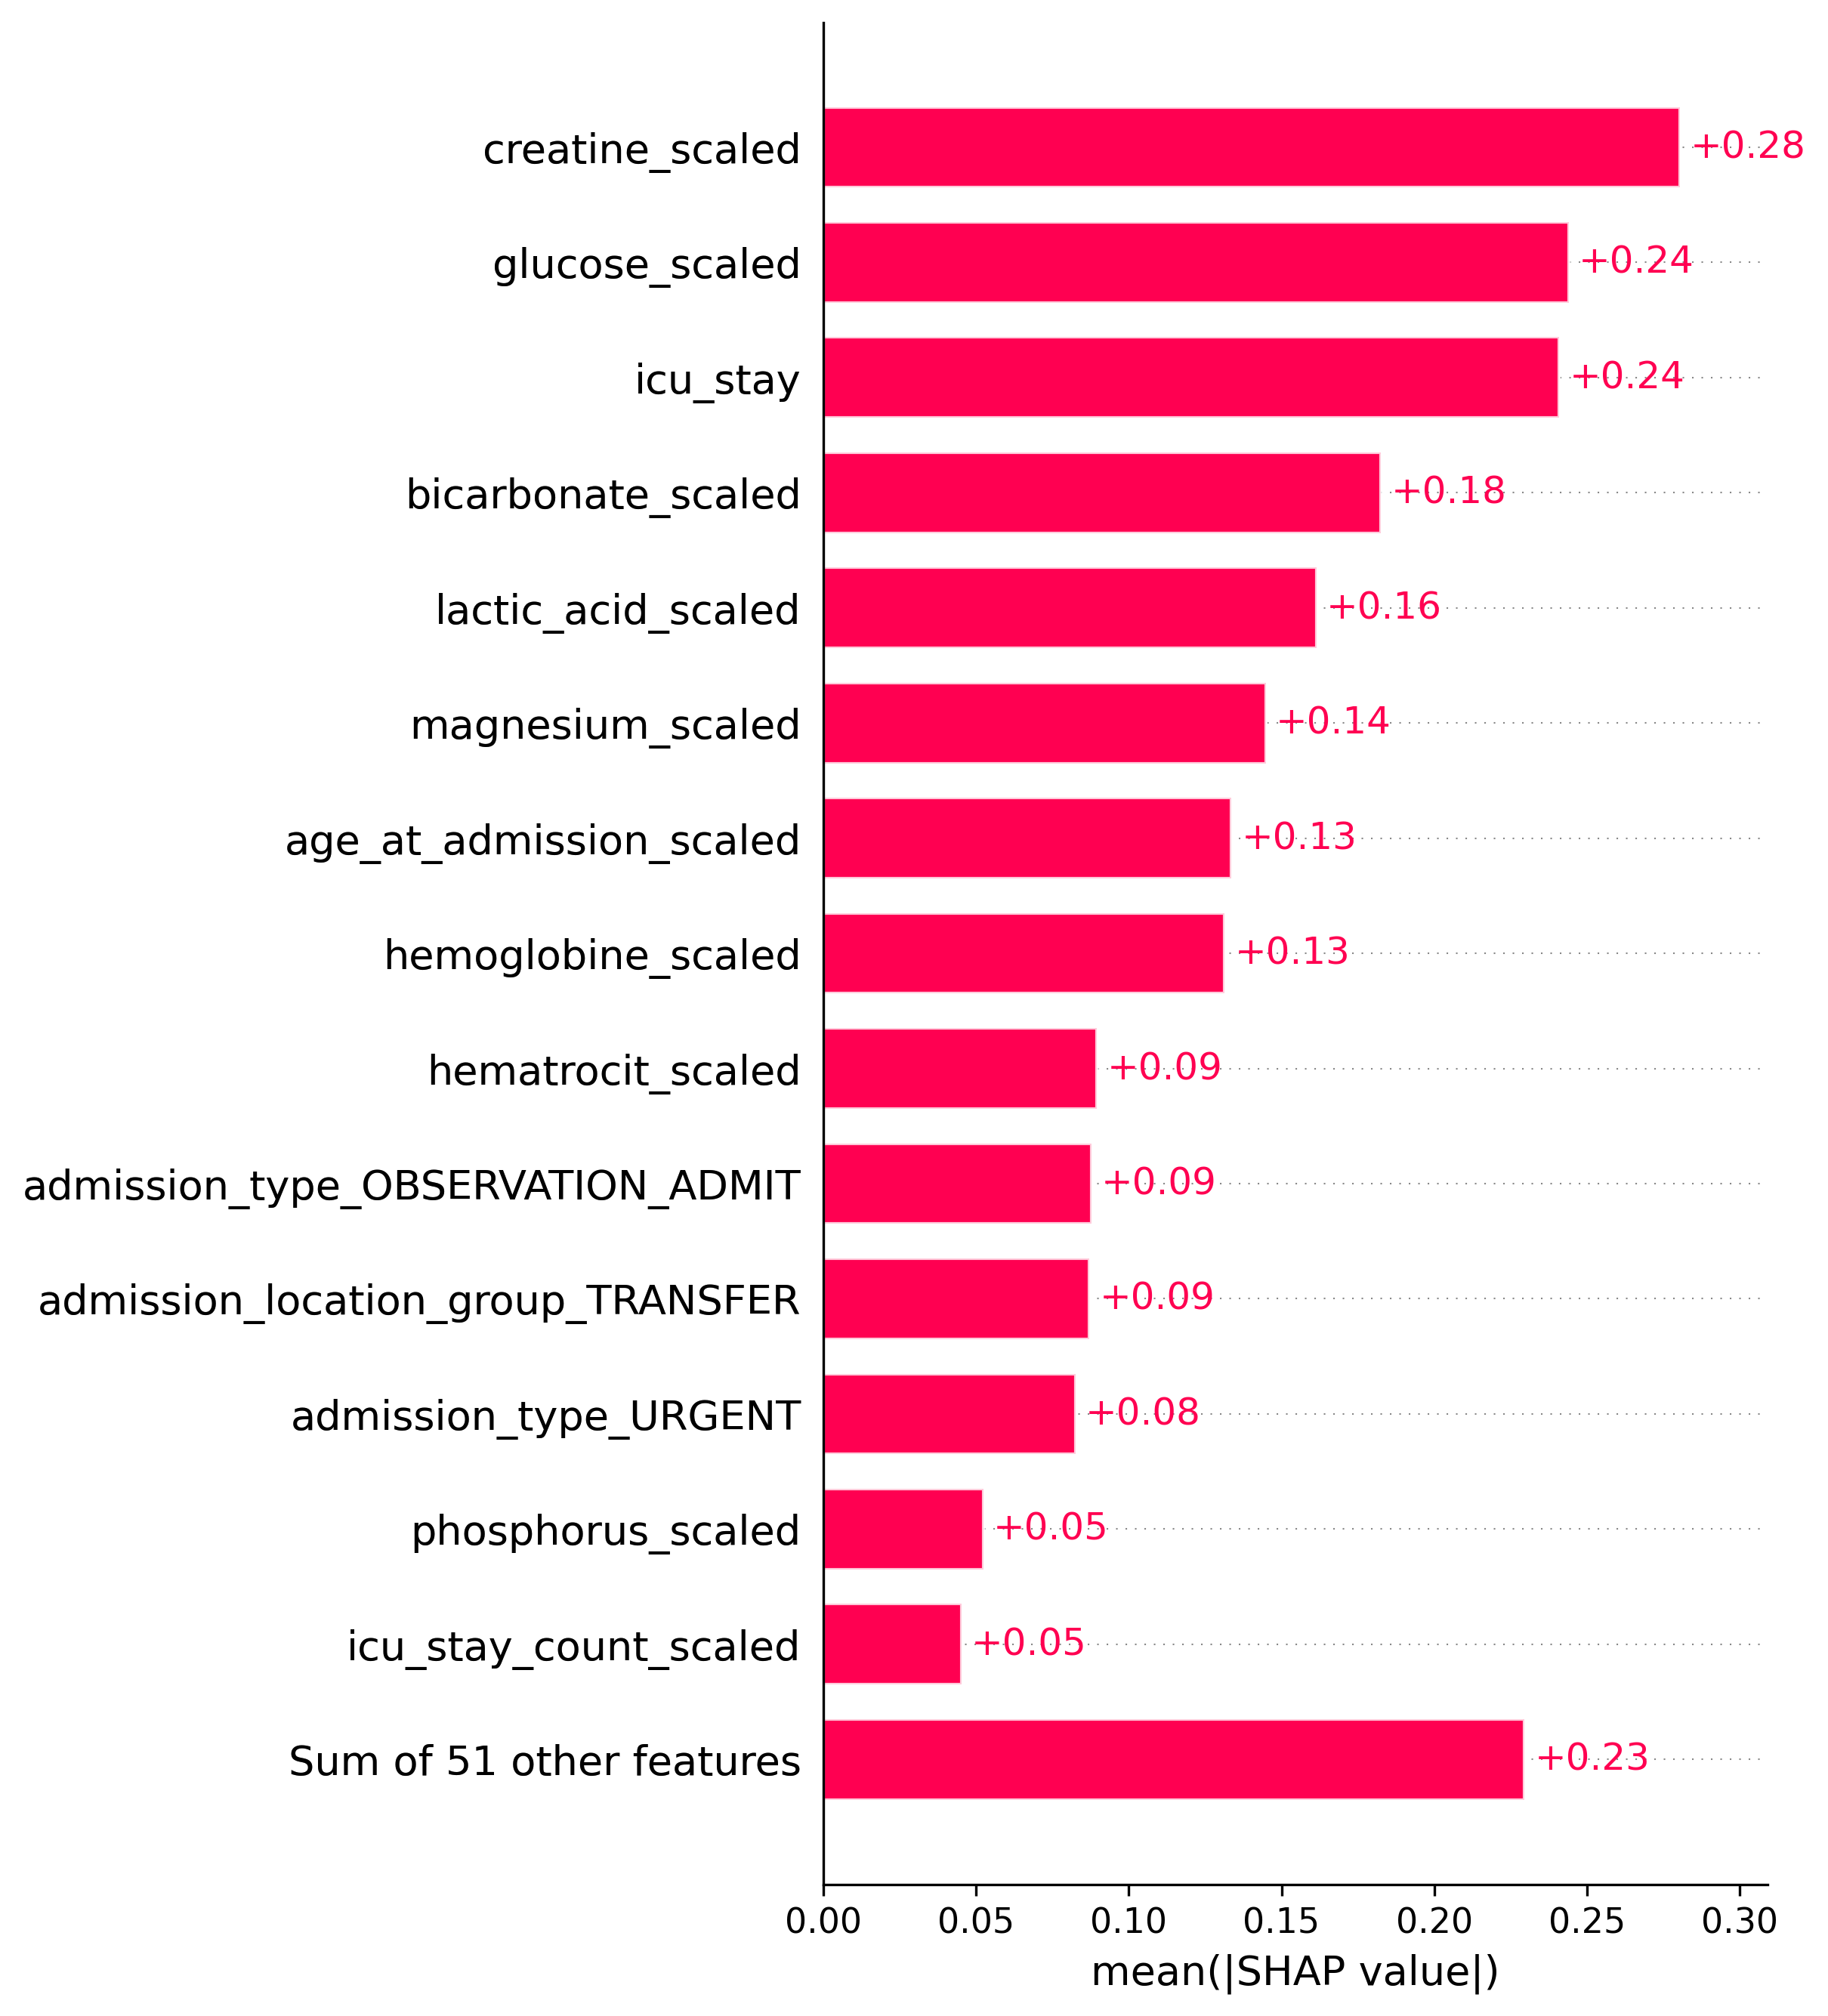
\includegraphics[width=0.6\textwidth]{fig_shap_bar_B.png}
\caption{Modelo~B: valor SHAP absoluto medio de las 15 variables más influyentes del aprendiz base XGBoost (conjunto de prueba).
Los nombres de las variables son los del cuaderno; el sufijo \texttt{\_scaled} indica la versión escalada de cada variable.}\label{fig:shap}
\end{figure}

En el conjunto de prueba, el AUC del ensamble apilado estuvo entre 0.86 y 0.95 en casi todos los subgrupos con al menos 10 ingresos
positivos (Tabla~\ref{tab:subgroup}); los intervalos de confianza fueron amplios y se solaparon entre grupos étnicos, categorías de
seguro y cuartiles de edad, por lo que no puede afirmarse ninguna diferencia entre ellos. No se evaluaron los subgrupos con menos de 10 positivos (grupos asiático,
hispano, indoamericano, blanco europeo e isleño del Pacífico; Medicare, otros seguros y seguro sin clasificar). La excepción clara
fueron los 94 ingresos con estancia en UCI, entre los cuales 36 (38\%) fueron casos de MMG y el AUC fue 0.655 (0.539--0.767): el modelo marcó
el 99\% de ellos, de modo que la estancia en UCI fue por sí sola un fuerte predictor de MMG pero el modelo no separó casos de
no casos dentro de este grupo. El desempeño fue similar en hospitalizaciones por parto (AUC 0.920) y no relacionadas con parto (0.913), aunque la AP fue tres
veces mayor en las primeras (0.646 frente a 0.221), reflejo de su mayor prevalencia. Todas las estimaciones por subgrupo son descriptivas, se basan en una sola partición de prueba y no
constituyen una evaluación formal de equidad.

\begin{table}[H]
\caption{Modelo~B: desempeño del ensamble apilado en el conjunto de prueba por subgrupo. Solo se muestran los subgrupos con al menos 10 ingresos positivos.
Los grupos de edad corresponden a los cuartiles de la edad escalada, aproximadamente $\leq$28, 29--32, 33--36 y $\geq$37 años. Las etiquetas de grupo étnico son las del cuaderno.\label{tab:subgroup}}
\small
\begin{tabularx}{\textwidth}{llccCc}
\toprule
\textbf{Dimensión} & \textbf{Subgrupo} & \textbf{Ingresos} & \textbf{Casos de MMG} & \textbf{AUC (IC 95\%)} & \textbf{AP}\\
\midrule
Grupo étnico & AFRO\_DESC & 1{,}285 & 28 & 0.866 (0.769--0.946) & 0.304\\
 & UNKNOWN & 619 & 17 & 0.944 (0.865--0.984) & 0.532\\
 & WHITE\_USA & 2{,}092 & 39 & 0.921 (0.868--0.965) & 0.355\\
Seguro & Medicaid & 1{,}731 & 32 & 0.902 (0.820--0.967) & 0.430\\
 & Privado & 3{,}194 & 60 & 0.923 (0.878--0.963) & 0.405\\
Edad & $\leq$28 años & 1{,}312 & 20 & 0.884 (0.773--0.968) & 0.351\\
 & 29--32 años & 1{,}271 & 18 & 0.940 (0.862--0.986) & 0.317\\
 & 33--36 años & 1{,}333 & 29 & 0.953 (0.917--0.982) & 0.473\\
 & $\geq$37 años & 1{,}232 & 28 & 0.860 (0.763--0.949) & 0.404\\
Estancia en UCI & Sí & 94 & 36 & 0.655 (0.539--0.767) & 0.609\\
 & No & 5{,}054 & 59 & 0.873 (0.815--0.929) & 0.219\\
Hospitalización & Parto & 1{,}802 & 58 & 0.920 (0.874--0.963) & 0.646\\
 & No parto & 3{,}346 & 37 & 0.913 (0.851--0.960) & 0.221\\
\bottomrule
\end{tabularx}
\end{table}

%--------------------------------------------------------------------
\section{Discusión}\label{sec:discussion}
%--------------------------------------------------------------------
\textbf{La mortalidad no es un objetivo de modelamiento con este tamaño de muestra.} Con 41 muertes,
valores de AUC con validación cruzada de 0.76--0.86 coexistieron con AP de 0.05--0.19, con
desviaciones estándar de la AP del mismo orden que las medias y con conclusiones en el conjunto de prueba
sustentadas en ocho muertes. Por tanto, una clasificación de los cinco algoritmos no es
confiable: por ejemplo, LR ocupó el segundo lugar en AUC en el conjunto de prueba (0.854) pero tuvo la menor AP en ese conjunto (0.031) y el menor
AUC y AP con validación cruzada (0.758 y 0.049), mientras que XGB tuvo la mayor AP en el conjunto de prueba (0.278)
pero una AP con validación cruzada (0.165) inferior a la de ET (0.190). Nuestros resultados
respaldan la recomendación de reportar métricas de precisión--sensibilidad y la
dispersión por partición para desenlaces raros~\cite{Marshall2023Imbalance,Saito2015PR}.

\textbf{La MMG es un sustituto más estable, pero ruidoso.} Una clase positiva once
veces mayor produjo valores de AUC en el conjunto de prueba de 0.889--0.913 con una dispersión estrecha entre
algoritmos, un ensamble apilado que fue el mejor tanto en AUC como en AP en el conjunto de prueba y con validación cruzada
(0.904 $\pm$ 0.020 y 0.419 $\pm$ 0.050, con desviaciones estándar del AUC entre particiones de aproximadamente una
tercera parte de las del Modelo~A), y un balance precisión--sensibilidad que puede discutirse clínicamente.
En términos de ordenamiento, el 5\% superior de los ingresos contuvo el 68\% de los casos de MMG con un valor predictivo positivo de 0.25
(\emph{lift} 13.6). Deben señalarse con claridad dos limitaciones.
Primero, la etiqueta de MMG se basa en CIE; la codificación CIE-10 mostró
baja sensibilidad y bajo valor predictivo positivo en un estudio de validación con
historias clínicas~\cite{Boulet2024ICD10SMM}, de modo que nuestros positivos son una aproximación administrativa, y
el modelo podría aprender en parte patrones de codificación y de intensidad de la atención. Esto también
probablemente explica la alta tasa de MMG en las hospitalizaciones por parto. Segundo, los principales
predictores del Modelo~B fueron creatinina, glucosa, bicarbonato y magnesio,
relacionados con el trastorno renal y metabólico; dado que la insuficiencia renal aguda es el
indicador más frecuente (180 ingresos), parte de la señal refleja
anomalías de laboratorio que coocurren con la definición del desenlace en lugar de
anticiparlo. Usar el valor más temprano disponible mitiga, pero no elimina, esta
preocupación, y no se impuso una temporalidad prospectiva de los predictores respecto del evento. El análisis SHAP y la auditoría por subgrupos apuntan en la misma dirección: la estancia en UCI y el ácido láctico
figuraron entre los predictores más influyentes, y el AUC fue el menor (0.655) en los 94 ingresos de prueba con estancia en UCI, entre los cuales
36 fueron casos de MMG y el modelo marcó el 99\%; por tanto, la estancia en UCI es en sí misma un fuerte marcador de MMG, pero el modelo no
separa casos de no casos entre los pacientes críticos. Las diferencias entre grupos étnicos, de seguro y de edad no se distinguieron del ruido muestral
(intervalos solapados basados en 17 a 60 positivos por subgrupo), y no puede hacerse ninguna afirmación sobre equidad a partir de ellas.

\textbf{Sobremuestreo y política de valores atípicos.} SMOTE no mejoró las métricas basadas
en precisión en ninguno de los dos modelos (AP del apilamiento de 0.156 a 0.168 en el Modelo~A y de 0.419 a 0.406 en el Modelo~B) y desplazó el
punto de operación de forma impredecible (sensibilidad de XGBoost en el Modelo~B de 0.758 a 0.964 con un F1 de 0.047), en línea con la evidencia de que las correcciones del desbalance pueden perjudicar la calibración
y no necesariamente mejoran la discriminación~\cite{vandenGoorbergh2022Harm}.
Reemplazar la eliminación de filas por la winsorización preservó todos los casos positivos;
conservarlos importa más que la pulcritud geométrica de la distribución de las variables,
ya que eliminar valores extremos de laboratorio remueve precisamente a los
pacientes más graves.

\textbf{Limitaciones.} (i) Datos de un solo centro y sin validación externa. (ii)
El Modelo~A incluye los 26 indicadores de grupos diagnósticos mientras que el Modelo~B los excluye; los
dos modelos no son, por tanto, estrictamente comparables en sus conjuntos de predictores. Retirar los indicadores del
Modelo~A redujo su AUC con validación cruzada de 0.857 a 0.725 y su AP de 0.156 a 0.013, de modo que su
desempeño con los grupos depende de variables derivadas de los diagnósticos del propio ingreso, que podrían
reflejar el curso clínico que conduce a la muerte en lugar de anticiparlo. (iii) Los valores de imputación y los escaladores
se ajustaron antes de la división entrenamiento/prueba, y la validación cruzada reajusta
hiperparámetros ajustados sobre la partición de entrenamiento, lo que puede hacer que las estimaciones sean ligeramente
optimistas. (iv) La etiqueta de MMG basada en CIE y las variables de laboratorio y de UCI pueden ser en parte concurrentes con el
evento (no se impuso la temporalidad de los predictores respecto del evento). (v) El desenlace de
mortalidad captura solo las muertes registradas por el hospital; las muertes posteriores al alta no
se observan. (vi) Las métricas con el umbral predeterminado de 0.5 se muestran por transparencia;
las probabilidades brutas fueron 13.5 veces (Modelo~B) y 238 veces (Modelo~A) mayores que la
prevalencia observada debido a la ponderación de clases~\cite{NiculescuMizil2005Probabilities,vandenGoorbergh2022Harm,VanCalster2019Calibration}; la recalibración a posteriori las corrigió, pero los mapas de calibración se
estimaron en la misma cohorte mediante validación cruzada repetida y no se han validado externamente, la regresión isotónica fue inestable en el Modelo~A con 41 eventos,
y no se optimizó el umbral. (vii) MIMIC-IV no es un registro obstétrico y
puede diferir de la población de los servicios obstétricos de
otros sistemas de salud. Los modelos son prototipos de investigación y no deben orientar
decisiones clínicas individuales.

%--------------------------------------------------------------------
\section{Implicaciones y trabajo futuro}\label{sec:implications}
%--------------------------------------------------------------------
\textbf{Implicaciones para la práctica.} Los resultados no respaldan el uso de ninguno de los modelos
para decisiones individuales. Sí indican cómo debería diseñarse una herramienta de riesgo materno:
como una clasificación de ingresos para revisión y no como un clasificador con un umbral predeterminado,
con la proporción de ingresos señalados elegida por un panel clínico a la luz del balance entre sensibilidad
y precisión, y con los riesgos absolutos recalibrados antes de mostrarse. Cualquier punto de
operación o acción desencadenada por una herramienta de este tipo en la atención obstétrica requiere validación
por un responsable humano autorizado.

\textbf{Vigilancia en lugar de predicción.} Dado que las categorías de MMG son
clínicamente distintas (renal, hemorrágica, respiratoria y otras), y que casi una cuarta parte
de los ingresos con MMG involucra más de una categoría, un hospital podría usar las mismas
variables para monitorear la carga de MMG por categoría y para revisar casos, aunque la predicción
individual siga siendo imperfecta.

\textbf{Consideraciones éticas y gobernanza.} Merecen mención explícita cuatro asuntos. Primero, los datos provienen de un único centro médico académico de
Estados Unidos y se obtuvieron bajo el acuerdo de uso de datos credencializado de PhysioNet, que prohíbe la reidentificación y el intercambio de datos
crudos con terceros sin credenciales; cualquier reutilización de estos modelos con otros datos de pacientes requiere su propia autorización y revisión ética.
Segundo, respecto del sesgo algorítmico, la auditoría por subgrupos (Tabla~\ref{tab:subgroup}) fue descriptiva y no pudo evaluar varios grupos étnicos y categorías de seguro por falta de eventos; los menores
AUC se observaron en el grupo AFRO\_DESC (0.866) y, sobre todo, entre los ingresos con estancia en UCI (0.655), y las predicciones pueden ser menos confiables para los
grupos ya subrepresentados en los datos de entrenamiento~\cite{Obermeyer2019Bias,Rajkomar2018Fairness}. Tercero, respecto de la transparencia, los valores SHAP describen asociaciones aprendidas por el modelo y no
mecanismos causales, y un predictor destacado puede ser un sustituto de un factor no medido; una ficha del modelo (\emph{model card}) que documente el uso previsto, los datos, el desempeño por
subgrupos y las limitaciones conocidas~\cite{Mitchell2019ModelCards} sería un requisito mínimo para cualquier publicación de estos modelos. Cuarto, respecto de la supervisión humana, los modelos son prototipos de investigación y
no deben usarse en la atención clínica; cualquier herramienta futura debería actuar como una ayuda no vinculante cuyas alertas los clínicos puedan anular y documentar, ir precedida de
validación prospectiva y revisión regulatoria en la jurisdicción aplicable, y monitorearse tras su despliegue para detectar deriva en la discriminación y la calibración (por ejemplo, con el AUC y el puntaje de Brier móviles), en
conjunto y por subgrupos.

\textbf{Trabajo futuro.} De las limitaciones se derivan cinco direcciones. (i)~Validación externa
en otras cohortes hospitalarias, en particular servicios obstétricos, para comprobar si la
señal impulsada por el laboratorio se generaliza; cuando no es posible reunir datos a nivel de paciente, el aprendizaje federado podría permitir el
entrenamiento y la validación multicéntricos sin compartir registros~\cite{Rieke2020Federated,Dayan2021Federated}. (ii)~Validación de la etiqueta de MMG basada en CIE frente a
la revisión de historias clínicas en una muestra, para estimar su sensibilidad y valor predictivo positivo
reales en esta cohorte. (iii)~Restricción de los predictores a valores registrados antes del evento, lo que convertiría el
modelo de MMG en un verdadero modelo de alerta temprana. (iv)~Validación externa de los mapas de recalibración y
análisis de curvas de decisión~\cite{Vickers2006DCA}. (v)~Un modelo multiclase secundario que prediga la categoría primaria de MMG
entre los ingresos positivos, lo que responde a la pregunta clínicamente distinta de qué complicación
es más probable una vez que ocurre la MMG.

%--------------------------------------------------------------------
\section{Conclusiones}\label{sec:conclusions}
%--------------------------------------------------------------------
En 25{,}736 ingresos obstétricos de MIMIC-IV, la muerte materna registrada en el ámbito hospitalario
(41 eventos) no pudo modelarse con una precisión confiable, mientras que la MMG (475 eventos)
permitió una evaluación estable, con un ensamble apilado que alcanzó un AUC de
0.913 y una AP de 0.384 en el conjunto de prueba, confirmadas por validación cruzada (0.904 y 0.419); el 5\% superior de los ingresos
según la probabilidad predicha contuvo el 68\% de los casos de MMG. La discriminación aparente para mortalidad dependió en gran parte de los indicadores de grupos
diagnósticos, las probabilidades brutas de ambos modelos no estuvieron calibradas (el escalamiento de Platt las corrigió) y el desempeño fue menor entre los ingresos con estancia en UCI. La ponderación de clases
fue preferible a SMOTE, y la winsorización protegió a los casos positivos de ser eliminados. El trabajo futuro debería validar estos modelos
en cohortes independientes, incluida la recalibración, y definir umbrales para un caso de uso de apoyo a la decisión,
y evaluar la tarea multiclase secundaria de predecir la categoría de MMG.

\vspace{6pt}
\authorcontributions{Conceptualización, E.G.J. y J.D.M.D.;
metodología, E.G.J.; software, E.G.J.; validación, E.G.J.;
análisis formal, E.G.J.; investigación, E.G.J.; curación de datos, E.G.J.;
redacción---preparación del borrador original, E.G.J.;
redacción---revisión y edición, E.G.J. y J.D.M.D.; visualización, E.G.J.;
supervisión, J.D.M.D.; obtención de financiación, E.G.J. Todos los autores han leído y aceptado la versión publicada
del manuscrito.}

\funding{Esta investigación fue apoyada por el programa Becas de Excelencia Doctoral
del Bicentenario, financiado por el Fondo de Ciencia, Tecnolog\'ia
e Innovaci\'on del Sistema General de Regal\'ias (FCTeI-SGR) y
administrado por el Ministerio de Ciencia, Tecnolog\'ia e Innovaci\'on (Minciencias) de Colombia.
Este apoyo se brindó a través del BPIN~2020000100287, por medio de la Universidad
del Norte, Barranquilla, Colombia, como institución ejecutora.}

\institutionalreview{Se renunció a la revisión y aprobación ética de este
estudio debido a la naturaleza retrospectiva, totalmente anonimizada y de uso secundario
de la base de datos MIMIC-IV. La recolección original y la
anonimización de los datos fueron revisadas y aprobadas por el
Comité de Ética Institucional (IRB) del Beth Israel Deaconess Medical Center
(BIDMC), que concedió una exención del consentimiento informado para la creación y
el intercambio de la base de datos~\cite{Johnson2023MIMICIV}.}

\informedconsent{El Comité de Ética Institucional del Beth Israel Deaconess Medical Center
renunció al consentimiento de los pacientes para la recolección original de la base de datos
MIMIC-IV, debido a su naturaleza retrospectiva y totalmente anonimizada~\cite{Johnson2023MIMICIV}.
Los autores no reclutaron directamente a ningún participante.}

\dataavailability{Los datos clínicos utilizados en este estudio están disponibles en
la base de datos MIMIC-IV, pero existen restricciones para su disponibilidad:
se emplearon bajo un acuerdo de uso de datos y, por lo tanto, no pueden redistribuirse
públicamente. Los datos están disponibles a través de PhysioNet~\cite{Goldberger2000PhysioNet}
para cualquier investigador que complete la capacitación requerida y firme el
Acuerdo de Uso de Datos de Salud con Credenciales de PhysioNet
(\url{https://physionet.org/content/mimiciv/}). Los scripts SQL y los cuadernos
para la extracción de la cohorte, el preprocesamiento y el modelamiento están disponibles en
\url{https://github.com/khem777/maternal-smm-mimicIV}.}

\acknowledgments{Los autores agradecen al equipo de MIMIC-IV del Laboratorio
de Fisiología Computacional (MIT) y al Beth Israel Deaconess Medical
Center por mantener y proporcionar acceso abierto a la base de datos.
Los autores agradecen también a los cuatro expertos clínicos que, de forma voluntaria y sin compensación económica, participaron en la agrupación de los códigos diagnósticos y que solicitaron permanecer en el anonimato.}

\conflictsofinterest{Los autores declaran no tener conflictos de interés. Los financiadores no tuvieron ningún papel en el diseño del estudio, en la recolección, el análisis o la interpretación de los datos, en la redacción del manuscrito ni en la decisión de publicar los resultados.}

\abbreviations{Abreviaturas}{
\noindent
\begin{tabular}{@{}ll}
AA    & Aprendizaje automático (\emph{machine learning}) \\
AP    & Precisión promedio (\emph{average precision}) \\
AUC   & Área bajo la curva característica operativa del receptor \\
BIDMC & Beth Israel Deaconess Medical Center \\
CDC   & Centros para el Control y la Prevención de Enfermedades \\
CIE   & Clasificación Internacional de Enfermedades \\
ET    & Extra Trees \\
FAD   & Datos federalmente disponibles (\emph{Federally Available Data}) \\
HRSA  & Administración de Recursos y Servicios de Salud \\
LR    & Regresión logística \\
MIMIC & Medical Information Mart for Intensive Care \\
MMG   & Morbilidad materna grave (SMM, \emph{severe maternal morbidity}) \\
PR    & Precisión--sensibilidad (\emph{precision--recall}) \\
RF    & Random Forest \\
RIC   & Rango intercuartílico \\
ROC   & Característica operativa del receptor \\
SMOTE & Técnica de sobremuestreo de la minoría sintética \\
UCI   & Unidad de cuidados intensivos \\
VC    & Validación cruzada \\
VPP   & Valor predictivo positivo \\
XGB   & XGBoost (\emph{Extreme Gradient Boosting}) \\
\end{tabular}}

\begin{adjustwidth}{-\extralength}{0cm}
\reftitle{Referencias}
\bibliography{bib/bibliography_maternal}
\end{adjustwidth}

\end{document}
